% Präambel mit Einstellungen importieren
% Doctype and used packages
\documentclass[open=right, % Kapitel darf nur auf rechten Seite beginnen
    paper=A4,               % DIN-A4-Papier
    a4paper,                % DIN-A4-Papier
    12pt,                   % Schriftgöße
    headings=small,         % Kleine Überschriften
    headsepline=true,       % Trennlinie am Kopf der Seite
    footsepline=false,      % Keine Trennlinie am Fuß der Seite
    bibliography=totoc,     % Literaturverzeichnis in das Inhaltsverzeichnis aufnehmen
    twoside=on,             % Doppelseitiger Druck - auf off stellen für einseitig
    DIV=7,                  % Verhältnis der Ränder zum bedruckten Bereich
    chapterprefix=true,     % Kapitel x vor dem Kapitelnamen
    cleardoublepage=plain]{scrbook}

% Pakete einbinden, die benötigt werden
\usepackage{scrpage2}
\usepackage[utf8]{inputenc}       % Dateien in UTF-8 benutzen
\usepackage[T1]{fontenc}          % Zeichenkodierung
\usepackage{graphicx}             % Bilder einbinden
\usepackage[main=ngerman, english]{babel}       % Deutsch und Englisch unterstützen
\usepackage{xcolor}               % Color support
\usepackage{amsmath}              % Mathematische Formeln
\usepackage{amsfonts}             % Mathematische Zeichensätze
\usepackage{amssymb}              % Mathematische Symbole
\usepackage{float}                % Fließende Objekte (Tabellen, Grafiken etc.)
\usepackage{booktabs}             % Korrekter Tabellensatz
\usepackage[printonlyused]{acronym}  % Abkürzungsverzeichnis [nur verwendete Abkürzungen]
\usepackage{makeidx}              % Sachregister
\usepackage{listings}             % Source Code listings
\usepackage{listingsutf8}         % Listings in UTF8
\usepackage[hang,font={sf,footnotesize},labelfont={footnotesize,bf}]{caption} % Beschriftungen
\usepackage[scaled]{helvet}       % Schrift Helvetia laden
\usepackage[absolute]{textpos}	  % Absolute Textpositionen (für Deckblatt)
\usepackage{calc}                 % Berechnung von Positionen
\usepackage{blindtext}            % Blindtexte
\usepackage[bottom=40mm,left=35mm,right=35mm,top=30mm]{geometry} % Ränder ändern
\usepackage{setspace}             % Abstände korrigieren
\usepackage{ifthen}               % Logische Bedingungen mit if-then-else
\usepackage{scrhack}              % Get rid of tocbasic warnings
\usepackage[pagebackref=false,german]{hyperref}  % Hyperlinks
\usepackage[all]{hypcap}          % Korrekte Verlinkung von Floats
\usepackage[autostyle=true,german=quotes]{csquotes}   % Zitate
\usepackage[backend=biber,
  isbn=false,                     % ISBN nicht anzeigen, gleiches geht mit nahezu allen anderen Feldern
  sortlocale=de_DE,               % Sortierung der Einträge für Deutsch
  %sortlocale=en_US,              % Sortierung der Einträge für Englisch
  autocite=inline,                % regelt Aussehen für \autocite (inline=\parancite)
  hyperref=true,                  % Hyperlinks für Ziate
  %style=ieee                     % Zitate als Zahlen [1]
  %style=alphabetic               % Zitate als Kürzel und Jahr [Ein05]
  style=authoryear                % Zitate Author und Jahr [Einstein (1905)]
]{biblatex}                       % Literaturverwaltung
\usepackage{rotating}             % Seiten drehen
\usepackage{harveyballs}          % Harveyballs

\setlength{\bibitemsep}{1em}     % Abstand zwischen den Literaturangaben
\setlength{\bibhang}{2em}        % Einzug nach jeweils erster Zeile

% Trennung von URLs im Literaturverzeichnis (große Werte [> 10000] verhindern die Trennung)
\defcounter{biburlnumpenalty}{10} % Strafe für Trennung in URL nach Zahl
\defcounter{biburlucpenalty}{500}  % Strafe für Trennung in URL nach Großbuchstaben
\defcounter{biburllcpenalty}{500}  % Strafe für Trennung in URL nach Kleinbuchstaben

% Farben definieren
\definecolor{linkblue}{RGB}{0, 0, 100}
\definecolor{linkblack}{RGB}{0, 0, 0}
\definecolor{comment}{RGB}{63, 127, 95}
\definecolor{darkgreen}{RGB}{14, 144, 102}
\definecolor{darkblue}{RGB}{0,0,168}
\definecolor{darkred}{RGB}{128,0,0}
\definecolor{javadoccomment}{RGB}{0,0,240}

% Einstellungen für das Hyperlink-Paket
\hypersetup{
    colorlinks=true,      % Farbige links verwenden
%    allcolors=linkblue,
    linktoc=all,          % Links im Inhaltsverzeichnis
    linkcolor=linkblack,  % Querverweise
    citecolor=linkblack,  % Literaturangaben
	filecolor=linkblack,  % Dateilinks
	urlcolor=linkblack    % URLs
}

% Einstellungen für Quelltexte
\lstset{
      xleftmargin=0.2cm,
      basicstyle=\footnotesize\ttfamily,
      keywordstyle=\color{darkgreen},
      identifierstyle=\color{darkblue},
      commentstyle=\color{comment},
      stringstyle=\color{darkred},
      tabsize=2,
      lineskip={2pt},
      columns=flexible,
      inputencoding=utf8,
      captionpos=b,
      breakautoindent=true,
	  breakindent=2em,
	  breaklines=true,
	  prebreak=,
	  postbreak=,
      numbers=none,
      numberstyle=\tiny,
      showspaces=false,      % Keine Leerzeichensymbole
      showtabs=false,        % Keine Tabsymbole
      showstringspaces=false,% Leerzeichen in Strings
      morecomment=[s][\color{javadoccomment}]{/**}{*/},
      literate={Ö}{{\"O}}1 {Ä}{{\"A}}1 {Ü}{{\"U}}1 {ß}{{\ss}}2 {ü}{{\"u}}1 {ä}{{\"a}}1 {ö}{{\"o}}1
}

\urlstyle{same}

% Einstellungen für Überschriften
\renewcommand*{\chapterformat}{%
  \Large\chapapp~\thechapter   % Große Schrift
  \vspace{0.3cm}               % Abstand zum Titel des Kapitels
}

% Abstände für die Überschriften setzen
\renewcommand{\chapterheadstartvskip}{\vspace*{2.6cm}}
\renewcommand{\chapterheadendvskip}{\vspace*{1.5cm}}

\RedeclareSectionCommand[
  beforeskip=-1.8\baselineskip,
  afterskip=0.25\baselineskip]{section}

\RedeclareSectionCommand[
  beforeskip=-1.8\baselineskip,
  afterskip=0.15\baselineskip]{subsection}

\RedeclareSectionCommand[
  beforeskip=-1.8\baselineskip,
  afterskip=0.15\baselineskip]{subsubsection}


% In der Kopfzeile nur die kurze Kapitelbezeichnung (ohne Kapitel davor)
\renewcommand*\chaptermarkformat{\thechapter\autodot\enskip}
\automark[chapter]{chapter}

% Einstellungen für Schriftarten
\setkomafont{pagehead}{\normalfont\sffamily}
\setkomafont{pagenumber}{\normalfont\sffamily}
\setkomafont{paragraph}{\sffamily\bfseries\small}
\setkomafont{subsubsection}{\sffamily\itshape\bfseries\small}
\addtokomafont{footnote}{\footnotesize}
\setkomafont{chapter}{\LARGE\selectfont\bfseries}

% Wichtige Abstände
\setlength{\parskip}{0.2cm}  % 2mm Abstand zwischen zwei Absätzen
\setlength{\parindent}{0mm}  % Absätze nicht einziehen
\clubpenalty = 10000         % Keine "Schusterjungen"
\widowpenalty = 10000        % Keine "Hurenkinder"
\displaywidowpenalty = 10000 % Keine "Hurenkinder"
\renewcommand{\footnotesize}{\fontsize{9}{10}\selectfont} % Größe der Fußnoten
\setlength{\footnotesep}{8pt} % Abstand zwischen den Fußnoten

% Index erzeugen
\makeindex

% Einfacher Font-Wechsel über dieses Makro
\newcommand{\changefont}[3]{
\fontfamily{#1} \fontseries{#2} \fontshape{#3} \selectfont}

% Eigenes Makro für Bilder
\newcommand{\bild}[3]{
\begin{figure}[h]
  \centering
  \includegraphics[width=#2]{#1}
  \caption{#3}
  \label{#1}
\end{figure}}

% Wo liegt Sourcecode?
\newcommand{\srcloc}{src/}

% Wo sind die Bilder?
\graphicspath{{bilder/}}

% Makros für typographisch korrekte Abkürzungen
\newcommand{\zb}[0]{z.\,B.\ }
\newcommand{\dahe}[0]{d.\,h.\ }
\newcommand{\ua}[0]{u.\,a.\ }

% Flags für Veröffentlichung und Sperrvermerk
\newboolean{hsmapublizieren}
\newboolean{hsmasperrvermerk}


% Dokumenteninfos importieren
% -------------------------------------------------------
% Daten für die Arbeit
% Wenn hier alles korrekt eingetragen wurde, wird das Titelblatt
% automatisch generiert. D.h. die Datei titelblatt.tex muss nicht mehr
% angepasst werden.

\newcommand{\hsmasprache}{de} % de oder en für Deutsch oder Englisch
% Für korrekt sortierte Literatureinträge, noch preambel.tex anpassen
% und zwar bei \usepackage[main=ngerman, english]{babel},
% \usepackage[pagebackref=false,german]{hyperref}
% und \usepackage[autostyle=true,german=quotes]{csquotes}

% Titel der Arbeit auf Deutsch
\newcommand{\hsmatitelde}{Analyse der Netzwerkkommunikation in Industrie 4.0 Umgebungen und Erweiterung einer protoypischen Security Testumgebung zur Darstellung von Bedrohungsfaktoren}

% Titel der Arbeit auf Englisch
\newcommand{\hsmatitelen}{TODO - Title EN}

% Weitere Informationen zur Arbeit
\newcommand{\hsmaort}{Mannheim} % Ort
\newcommand{\hsmaautorvname}{Philipp} % Vorname(n)
\newcommand{\hsmaautornname}{Minges} % Nachname(n)
\newcommand{\hsmadatum}{15.07.2018} % Datum der Abgabe
\newcommand{\hsmajahr}{2018} % Jahr der Abgabe
\newcommand{\hsmafirma}{Hochschule Mannheim, Mannheim} % Firma bei der die Arbeit durchgeführt wurde
\newcommand{\hsmabetreuer}{Prof. Sachar Paulus, Hochschule Mannheim} % Betreuer an der Hochschule
\newcommand{\hsmazweitkorrektor}{Prof. Dr. Maximilian Hauske, Hochschule Mannheim} % Betreuer im Unternehmen oder Zweitkorrektor
\newcommand{\hsmafakultaet}{I} % I für Informatik
\newcommand{\hsmastudiengang}{IB} % IB IMB UIB IM MTB

% Zustimmung zur Veröffentlichung
\setboolean{hsmapublizieren}{true}   % Einer Veröffentlichung wird zugestimmt
\setboolean{hsmasperrvermerk}{false} % Die Arbeit hat keinen Sperrvermerk

% -------------------------------------------------------
% Abstract

% Kurze (maximal halbseitige) Beschreibung, worum es in der Arbeit geht auf Deutsch
\newcommand{\hsmaabstractde}{Nach der Einführung des Begriffs „Industrie 4.0“ im Jahr 2011 und dem gleichzeitigen Start der 4. industriellen Revolution werden Kommunikationsnetze in der Industrie immer mehr zur Automatisierung der Produktion von Gütern oder zum unternehmensinternen sowie -externen Datenaustausch genutzt. Um diese Echtzeitkommunikation oder auch Möglichkeiten der Fernwartung zu gewährleisten, werden immer mehr Anlagen mit Netzwerkzugängen ausgestattet. Die Kommunikation der Industrie 4.0 Netze und Systeme findet unternehmensübergreifend über einen unsicheren Kanal statt und kann somit ohne bereitgestellte Sicherheitsmaßnahmen genauso angegriffen werden, wie herkömmliche Heim- oder Büronetzwerke. Das Ziel dieser Arbeit ist es zum einen, die Netzwerkkommunikation zwischen Industrie 4.0 Komponenten anhand aktueller Standards zu analysieren, mögliche Angriffsvektoren darzustellen und deren Eintrittswahrscheinlichkeit sowie Schaden zu bewerten. Zum anderen wird ein vorhandenes Industrie 4.0 Security Testsystem anhand der gewonnenen Erkenntnisse im Bereich der Netzwerksicherheit zu Lehr- und Testzwecken prototypisch erweitert. TODO - neu Das Ziel dieser Arbeit ist es, die aus der }

% Kurze (maximal halbseitige) Beschreibung, worum es in der Arbeit geht auf Englisch

\newcommand{\hsmaabstracten}{TODO - Abstract EN}


% Literatur-Datenbank
\addbibresource{library.bib}

\begin{document}
\frontmatter

% Römische Ziffern für die "Front-Matter"
\setcounter{page}{0}
\changefont{ptm}{m}{n}  % Times New Roman für den Fließtext
\renewcommand{\rmdefault}{ptm}

% Titelblatt
% -------------------------------------------------------
% In dieser Datei sollten eigentlich keine Veränderungen mehr
% notwendig sein.
% -------------------------------------------------------

\thispagestyle{empty}

% Fakultäten der HS-Mannheim
% -------------------------------------------------------
\ifthenelse{\equal{\hsmafakultaet}{I}}%
  {\newcommand{\hsmafakultaetlangde}{Fakultät für Informatik}%
   \newcommand{\hsmafakultaetlangen}{Department of Computer Science}}{}

\ifthenelse{\equal{\hsmafakultaet}{E}}%
  {\newcommand{\hsmafakultaetlangde}{Fakultät für Elektrotechnik}%
   \newcommand{\hsmafakultaetlangen}{Department of Electrical Engineering}}{}

\ifthenelse{\equal{\hsmafakultaet}{S}}%
  {\newcommand{\hsmafakultaetlangde}{Fakultät für Sozialwesen}%
   \newcommand{\hsmafakultaetlangen}{Department of Social Work}}{}
   
\ifthenelse{\equal{\hsmafakultaet}{B}}%
  {\newcommand{\hsmafakultaetlangde}{Fakultät für Biotechnologie}%
   \newcommand{\hsmafakultaetlangen}{Department of Biotechnology}}{}

\ifthenelse{\equal{\hsmafakultaet}{D}}%
  {\newcommand{\hsmafakultaetlangde}{Fakultät für Gestaltung}%
   \newcommand{\hsmafakultaetlangen}{Department of Design}}{}

\ifthenelse{\equal{\hsmafakultaet}{M}}%
  {\newcommand{\hsmafakultaetlangde}{Fakultät für Maschinenbau}%
   \newcommand{\hsmafakultaetlangen}{Department of Mechanical Engineering}}{}

\ifthenelse{\equal{\hsmafakultaet}{N}}%
  {\newcommand{\hsmafakultaetlangde}{Fakultät für Informationstechnik}%
   \newcommand{\hsmafakultaetlangen}{Department of Information Technology}}{}
   
\ifthenelse{\equal{\hsmafakultaet}{W}}%
  {\newcommand{\hsmafakultaetlangde}{Fakultät für Wirtschaftsingenieurwesen}%
   \newcommand{\hsmafakultaetlangen}{Department of Engineering and Management}}{}
   
\ifthenelse{\equal{\hsmafakultaet}{C}}%
  {\newcommand{\hsmafakultaetlangde}{Fakultät für Verfahrens- und Chemietechnik}%
   \newcommand{\hsmafakultaetlangen}{Department of Chemical Process Engineering}}{}
   

\ifthenelse{\equal{\hsmastudiengang}{IB}}%
  {\newcommand{\hsmastudienganglangde}{Informatik}%
  \newcommand{\hsmastudienganglangen}{Computer Science}%
  \newcommand{\hsmatypde}{Bachelor-Thesis}%
  \newcommand{\hsmatypen}{Bachelor Thesis}%
  \newcommand{\hsmagrad}{\hsmabsc}}{}

\ifthenelse{\equal{\hsmastudiengang}{IMB}}%
  {\newcommand{\hsmastudienganglangde}{Medizinische Informatik}%
  \newcommand{\hsmastudienganglangen}{Medical Informatics}%
  \newcommand{\hsmatypde}{Bachelor-Thesis}%
  \newcommand{\hsmatypen}{Bachelor Thesis}%
  \newcommand{\hsmagrad}{\hsmabsc}}{}
  
\ifthenelse{\equal{\hsmastudiengang}{UIB}}%
  {\newcommand{\hsmastudienganglangde}{Unternehmens- und Wirtschaftsinformatik}%
  \newcommand{\hsmastudienganglangen}{Enterprise Computing}%  
  \newcommand{\hsmatypde}{Bachelor-Thesis}%
  \newcommand{\hsmatypen}{Bachelor Thesis}%
  \newcommand{\hsmagrad}{\hsmabsc}}{}

\ifthenelse{\equal{\hsmastudiengang}{IM}}%
  {\newcommand{\hsmastudienganglangde}{Informatik}%
   \newcommand{\hsmastudienganglangen}{Computer Science}%
   \newcommand{\hsmatypde}{Master-Thesis}%
   \newcommand{\hsmatypen}{Master Thesis}%
   \newcommand{\hsmagrad}{\hsmamaster}}{}

\ifthenelse{\equal{\hsmastudiengang}{MEB}}%
  {\newcommand{\hsmastudienganglangde}{Mechatronik}%
   \newcommand{\hsmastudienganglangen}{Mechatronic}%
   \newcommand{\hsmatypde}{Bachelor-Thesis}%
   \newcommand{\hsmatypen}{Bachelor Thesis}%
   \newcommand{\hsmagrad}{\hsmabsc}}{}
   
\ifthenelse{\equal{\hsmastudiengang}{UB}}%
  {\newcommand{\hsmastudienganglangde}{Automatisierungstechnik}%
   \newcommand{\hsmastudienganglangen}{Automation Technology}%
   \newcommand{\hsmatypde}{Bachelor-Thesis}%
   \newcommand{\hsmatypen}{Bachelor Thesis}%
   \newcommand{\hsmagrad}{\hsmabsc}}{}
   
\ifthenelse{\equal{\hsmastudiengang}{ELB}}%
  {\newcommand{\hsmastudienganglangde}{Elektro- und Informationstechnik/Ingenieurpädagogik}%
   \newcommand{\hsmastudienganglangen}{Elektro- und Informationstechnik/Ingenieurpädagogik}%
   \newcommand{\hsmatypde}{Bachelor-Thesis}%
   \newcommand{\hsmatypen}{Bachelor Thesis}%
   \newcommand{\hsmagrad}{\hsmabsc}}{} 
   
\ifthenelse{\equal{\hsmastudiengang}{EBE}}%
  {\newcommand{\hsmastudienganglangde}{Energietechnik und erneuerbare Energien}%
   \newcommand{\hsmastudienganglangen}{Power Engineering ans Renewable Energies}%
   \newcommand{\hsmatypde}{Bachelor-Thesis}%
   \newcommand{\hsmatypen}{Bachelor Thesis}%
   \newcommand{\hsmagrad}{\hsmabsc}}{}

\ifthenelse{\equal{\hsmastudiengang}{TS}}%
  {\newcommand{\hsmastudienganglangde}{Translation Studies}%
   \newcommand{\hsmastudienganglangen}{Translation Studies}%
   \newcommand{\hsmatypde}{Bachelor-Thesis}%
   \newcommand{\hsmatypen}{Bachelor Thesis}%
   \newcommand{\hsmagrad}{\hsmabsc}}{}
  
\ifthenelse{\equal{\hsmastudiengang}{EM}}%
  {\newcommand{\hsmastudienganglangde}{Automatisierungs- und Energiesysteme}%
   \newcommand{\hsmastudienganglangen}{Automation and Energy Systems}%
   \newcommand{\hsmatypde}{Master-Thesis}%
   \newcommand{\hsmatypen}{Master Thesis}%
   \newcommand{\hsmagrad}{\hsmamaster}}{}
   
\ifthenelse{\equal{\hsmastudiengang}{ELM}}%
  {\newcommand{\hsmastudienganglangde}{Lehramt Ingenieurpädagogik}%
   \newcommand{\hsmastudienganglangen}{Lectureship Educational Engineering}%
   \newcommand{\hsmatypde}{Master-Thesis}%
   \newcommand{\hsmatypen}{Master Thesis}%
   \newcommand{\hsmagrad}{\hsmamaster}}{}
   
\ifthenelse{\equal{\hsmastudiengang}{SAB}}%
  {\newcommand{\hsmastudienganglangde}{Soziale Arbeit}%
   \newcommand{\hsmastudienganglangen}{Social Labour}%
   \newcommand{\hsmatypde}{Bachelor-Thesis}%
   \newcommand{\hsmatypen}{Bachelor Thesis}%
   \newcommand{\hsmagrad}{\hsmaba}}{}
   
\ifthenelse{\equal{\hsmastudiengang}{SAM}}%
  {\newcommand{\hsmastudienganglangde}{Soziale Arbeit}%
   \newcommand{\hsmastudienganglangen}{Social Labour}%
   \newcommand{\hsmatypde}{Master-Thesis}%
   \newcommand{\hsmatypen}{Master Thesis}%
   \newcommand{\hsmagrad}{\hsmamastera}}{}
   
\ifthenelse{\equal{\hsmastudiengang}{BB}}%
  {\newcommand{\hsmastudienganglangde}{Biotechnology}%
   \newcommand{\hsmastudienganglangen}{Biotechnology}%
   \newcommand{\hsmatypde}{Bachelor-Thesis}%
   \newcommand{\hsmatypen}{Bachelor Thesis}%
   \newcommand{\hsmagrad}{\hsmabsc}}{}
   
\ifthenelse{\equal{\hsmastudiengang}{BCB}}%
  {\newcommand{\hsmastudienganglangde}{Biologische Chemie}%
   \newcommand{\hsmastudienganglangen}{Biological Chemics}%
   \newcommand{\hsmatypde}{Bachelor-Thesis}%
   \newcommand{\hsmatypen}{Bachelor Thesis}%
   \newcommand{\hsmagrad}{\hsmabsc}}{}
   
\ifthenelse{\equal{\hsmastudiengang}{BMEBST}}%
  {\newcommand{\hsmastudienganglangde}{Biotechnology - Biomedical Science and Technology}%
   \newcommand{\hsmastudienganglangen}{Biotechnology - Biomedical Science and Technology}%
   \newcommand{\hsmatypde}{Master-Thesis}%
   \newcommand{\hsmatypen}{Master Thesis}%
   \newcommand{\hsmagrad}{\hsmamaster}}{}
   
\ifthenelse{\equal{\hsmastudiengang}{BMEBPD}}%
  {\newcommand{\hsmastudienganglangde}{Biotechnology - Bioprocess Development}%
   \newcommand{\hsmastudienganglangen}{Biotechnology - Bioprocess Development}%
   \newcommand{\hsmatypde}{Master-Thesis}%
   \newcommand{\hsmatypen}{Master Thesis}%
   \newcommand{\hsmagrad}{\hsmamaster}}{}
   
\ifthenelse{\equal{\hsmastudiengang}{BLSM}}%
  {\newcommand{\hsmastudienganglangde}{Life Science Management}%
   \newcommand{\hsmastudienganglangen}{Life Science Management}%
   \newcommand{\hsmatypde}{Master-Thesis}%
   \newcommand{\hsmatypen}{Master Thesis}%
   \newcommand{\hsmagrad}{\hsmamaster}}{}
   
\ifthenelse{\equal{\hsmastudiengang}{KDB}}%
  {\newcommand{\hsmastudienganglangde}{Kommunikationsdesign}%
   \newcommand{\hsmastudienganglangen}{Communication Design}%
   \newcommand{\hsmatypde}{Bachelor-Thesis}%
   \newcommand{\hsmatypen}{Bachelor Thesis}%
   \newcommand{\hsmagrad}{\hsmaba}}{}
   
\ifthenelse{\equal{\hsmastudiengang}{KDM}}%
  {\newcommand{\hsmastudienganglangde}{Kommunikationsdesign}%
   \newcommand{\hsmastudienganglangen}{Communication Design}%
   \newcommand{\hsmatypde}{Master-Thesis}%
   \newcommand{\hsmatypen}{Master Thesis}%
   \newcommand{\hsmagrad}{\hsmamastera}}{}
   
\ifthenelse{\equal{\hsmastudiengang}{MB}}%
  {\newcommand{\hsmastudienganglangde}{Maschinenbau}%
   \newcommand{\hsmastudienganglangen}{Mechanical Engineering}%
   \newcommand{\hsmatypde}{Bachelor-Thesis}%
   \newcommand{\hsmatypen}{Bachelor Thesis}%
   \newcommand{\hsmagrad}{\hsmabsc}}{}
   
\ifthenelse{\equal{\hsmastudiengang}{MM}}%
  {\newcommand{\hsmastudienganglangde}{Maschinenbau}%
   \newcommand{\hsmastudienganglangen}{Mechanical Engineering}%
   \newcommand{\hsmatypde}{Master-Thesis}%
   \newcommand{\hsmatypen}{Master Thesis}%
   \newcommand{\hsmagrad}{\hsmamaster}}{}
   
\ifthenelse{\equal{\hsmastudiengang}{NEB}}%
  {\newcommand{\hsmastudienganglangde}{Elektronik}%
   \newcommand{\hsmastudienganglangen}{Electronics}%
   \newcommand{\hsmatypde}{Bachelor-Thesis}%
   \newcommand{\hsmatypen}{Bachelor Thesis}%
   \newcommand{\hsmagrad}{\hsmabsc}}{}
   
\ifthenelse{\equal{\hsmastudiengang}{TIB}}%
  {\newcommand{\hsmastudienganglangde}{Technische Informatik}%
   \newcommand{\hsmastudienganglangen}{Technical Information Technology}%
   \newcommand{\hsmatypde}{Bachelor-Thesis}%
   \newcommand{\hsmatypen}{Bachelor Thesis}%
   \newcommand{\hsmagrad}{\hsmabsc}}{}
   
\ifthenelse{\equal{\hsmastudiengang}{MTB}}%
  {\newcommand{\hsmastudienganglangde}{Medizintechnik}%
   \newcommand{\hsmastudienganglangen}{Medical Technology}%
   \newcommand{\hsmatypde}{Bachelor-Thesis}%
   \newcommand{\hsmatypen}{Bachelor Thesis}%
   \newcommand{\hsmagrad}{\hsmabsc}}{}
   
\ifthenelse{\equal{\hsmastudiengang}{MTM}}%
  {\newcommand{\hsmastudienganglangde}{Medizintechnik}%
   \newcommand{\hsmastudienganglangen}{Medical Technology}%
   \newcommand{\hsmatypde}{Master-Thesis}%
   \newcommand{\hsmatypen}{Master Thesis}%
   \newcommand{\hsmagrad}{\hsmamaster}}{}
   
\ifthenelse{\equal{\hsmastudiengang}{NM}}%
  {\newcommand{\hsmastudienganglangde}{Informationstechnik}%
   \newcommand{\hsmastudienganglangen}{Informationstechnik}%
   \newcommand{\hsmatypde}{Master-Thesis}%
   \newcommand{\hsmatypen}{Master Thesis}%
   \newcommand{\hsmagrad}{\hsmamaster}}{}
   
\ifthenelse{\equal{\hsmastudiengang}{WB}}%
  {\newcommand{\hsmastudienganglangde}{Wirtschaftsingenieurwesen}%
   \newcommand{\hsmastudienganglangen}{Business Administration and Engineering}%
   \newcommand{\hsmatypde}{Bachelor-Thesis}%
   \newcommand{\hsmatypen}{Bachelor Thesis}%
   \newcommand{\hsmagrad}{\hsmabsc}}{}
   
\ifthenelse{\equal{\hsmastudiengang}{WM}}%
  {\newcommand{\hsmastudienganglangde}{Wirtschaftsingenieurwesen}%
   \newcommand{\hsmastudienganglangen}{Business Administration and Engineering}%
   \newcommand{\hsmatypde}{Master-Thesis}%
   \newcommand{\hsmatypen}{Master Thesis}%
   \newcommand{\hsmagrad}{\hsmamaster}}{}
   
\ifthenelse{\equal{\hsmastudiengang}{VB}}%
  {\newcommand{\hsmastudienganglangde}{Verfahrenstechnik}%
   \newcommand{\hsmastudienganglangen}{Process Engineering}%
   \newcommand{\hsmatypde}{Bachelor-Thesis}%
   \newcommand{\hsmatypen}{Bachelor Thesis}%
   \newcommand{\hsmagrad}{\hsmabsc}}{}
   
\ifthenelse{\equal{\hsmastudiengang}{CB}}%
  {\newcommand{\hsmastudienganglangde}{Chemische Technik}%
   \newcommand{\hsmastudienganglangen}{Chemical Engineering}%
   \newcommand{\hsmatypde}{Bachelor-Thesis}%
   \newcommand{\hsmatypen}{Bachelor Thesis}%
   \newcommand{\hsmagrad}{\hsmabsc}}{}
   
\ifthenelse{\equal{\hsmastudiengang}{CM}}%
  {\newcommand{\hsmastudienganglangde}{Chemieingenieurwesen}%
   \newcommand{\hsmastudienganglangen}{Chemical Engineering}%
   \newcommand{\hsmatypde}{Master-Thesis}%
   \newcommand{\hsmatypen}{Master Thesis}%
   \newcommand{\hsmagrad}{\hsmamaster}}{}

\newcommand{\hsmabsc}{Bachelor of Science (B.Sc.)}
\newcommand{\hsmaba}{Bachelor of Arts (B.A.)}
\newcommand{\hsmamaster}{Master of Science (M.Sc.)}
\newcommand{\hsmamastera}{Master of Arts (M.A.)}
\newcommand{\hsmamasterba}{Master of Business Administration (MBA)}

\newcommand{\hsmakoerperschaftde}{Hochschule Mannheim}
\newcommand{\hsmakoerperschaften}{University of Applied Sciences Mannheim}

\newcommand{\hsmaautorbib}{\hsmaautornname, \hsmaautorvname} % Autor Nachname, Vorname
\newcommand{\hsmaautor}{\hsmaautorvname \ \hsmaautornname} % Autor Vorname Nachname

\ifthenelse{\equal{\hsmasprache}{de}}%
  {\newcommand{\hsmatyp}{\hsmatypde}%
   \newcommand{\hsmathesistype}{zur Erlangung des akademischen Grades \hsmagrad}%
   \newcommand{\hsmakoerperschaft}{\hsmakoerperschaftde}%
   \newcommand{\hsmastudiengangname}{Studiengang \hsmastudienganglangde}%
   \newcommand{\hsmastudienganglang}{\hsmastudienganglangde}%
   \newcommand{\hsmatitel}{\hsmatitelde}%
   \newcommand{\hsmatutor}{Betreuer}%
   \newcommand{\hsmafakultaetlang}{\hsmafakultaetlangde}%
   \newcommand{\hsmalistoftables}{Tabellenverzeichnis}%
   \newcommand{\hsmalistoffigures}{Abbildungsverzeichnis}%
   \newcommand{\hsmalistings}{Quellcodeverzeichnis}%
   \newcommand{\hsmaindex}{Index}%
   \newcommand{\hsmaabbreviations}{Abkürzungsverzeichnis}%   
   \selectlanguage{ngerman}}%
  {\newcommand{\hsmatyp}{\hsmatypen}%
   \newcommand{\hsmathesistype}{for the acquisition of the academic degree \hsmagrad}%
   \newcommand{\hsmakoerperschaft}{\hsmakoerperschaften}%
   \newcommand{\hsmastudiengangname}{Course of Studies: \hsmastudienganglang}%
   \newcommand{\hsmastudienganglang}{\hsmastudienganglangen}%
   \newcommand{\hsmatitel}{\hsmatitelen}%
   \newcommand{\hsmatutor}{Tutors}
   \newcommand{\hsmafakultaetlang}{\hsmafakultaetlangen}%
   \newcommand{\hsmalistoftables}{List of Tables}%
   \newcommand{\hsmalistoffigures}{List of Figures}%
   \newcommand{\hsmalistings}{Listings}%
   \newcommand{\hsmaindex}{Index}%
   \newcommand{\hsmaabbreviations}{List of Abbreviations}%
   \selectlanguage{english}}%


% Daten in die Standard-Felder von KOMA-Script eintragen
\titlehead{\hsmatyp\ in\  \hsmastudienganglang}
\subject{}
\title{\hsmatitel}
\author{\hsmaauthor}
\date{\small{\hsmadatum}}

% Daten für das fertige PDF-Dokument
\hypersetup{
  pdftitle={\hsmatitel},  % Titel des Dokuments
  pdfauthor={\hsmaautor},              % Autor
  pdfsubject={\hsmatyp\ in\ \hsmastudienganglang},                % Thema
  pdfkeywords={\hsmatitel}         % Schlüsselworte
}

\newlength{\bindekorrektur}
\newlength{\seitenanfang}
\newlength{\seitenbreite}
  
\setlength{\bindekorrektur}{-46mm}   % Korrektur der horizontalen Position
\setlength{\seitenanfang}{0mm}       % Korrektur der vertikalen Position
\setlength{\seitenbreite}{297mm}

\noindent
\includegraphics[width=7cm]{hsma-logo.pdf}\\

% Titel der Arbeit
\begin{textblock*}{128mm}(45mm,\seitenanfang + 62mm) % 4,5cm vom linken Rand und 6,0cm vom oberen Rand
  \centering\Large\sffamily
  \vspace{4mm} % Kleiner zusätzlicher Abstand oben für bessere Optik
  \textbf{\hsmatitel}
\end{textblock*}%

% Name
\begin{textblock*}{128mm}(45mm,\seitenanfang + 103mm)
  \centering\large\sffamily
  \hsmaautor
\end{textblock*}

% Thesis
\begin{textblock*}{\seitenbreite}(\bindekorrektur,\seitenanfang + 130mm)
  \centering\large\sffamily
  \hsmatyp\\
  \begin{small}\hsmathesistype \end{small}\\
  \vspace{2mm}
  \hsmastudiengangname
\end{textblock*}

% Fakultät
\begin{textblock*}{\seitenbreite}(\bindekorrektur,\seitenanfang + 165mm)
  \centering\large\sffamily
  \hsmafakultaetlang\\
  \vspace{2mm}
  \hsmakoerperschaft
\end{textblock*}

% Datum
\begin{textblock*}{\seitenbreite}(\bindekorrektur,\seitenanfang + 190mm)
  \centering\large 
  \textsf{\hsmadatum}
\end{textblock*}

% Firma
\begin{textblock*}{\seitenbreite}(\bindekorrektur,\seitenanfang + 215mm)
  \centering\large 
  %\textsf{Durchgeführt bei der Firma \hsmafirma}
\end{textblock*}

% Betreuer
\begin{textblock*}{\seitenbreite}(\bindekorrektur,\seitenanfang + 240mm)
  \centering\large\sffamily
  \hsmatutor \\
  \vspace{2mm}
  \hsmabetreuer\\
  \vspace{2mm}
  \hsmazweitkorrektor
\end{textblock*}

% Bibliographische Informationen
\null\newpage
\thispagestyle{empty}
  
\newcommand{\hsmabibde}{\begin{small}\textbf{\hsmaautorbib}: \\ \hsmatitelde \ / \hsmaautor. \ -- \\ \hsmatypde, \hsmaort : \hsmakoerperschaftde, \hsmajahr. \pageref{lastpage} Seiten.\end{small}}

\newcommand{\hsmabiben}{\begin{small}\textbf{\hsmaautorbib}: \\ \hsmatitelen \ / \hsmaautor. \ -- \\ \hsmatypen, \hsmaort : \hsmakoerperschaften, \hsmajahr. \pageref{lastpage} pages. \end{small}}

\ifthenelse{\equal{\hsmasprache}{de}}%
  {\hsmabibde \\ \vspace{0.5cm} \\ \hsmabiben}
  {\hsmabiben \\ \vspace{0.5cm} \\ \hsmabibde}


% Erklärung
\clearpage\setcounter{page}{1}
\thispagestyle{empty}
\textsf{\large\textbf{Erklärung}}

Hiermit erkläre ich, dass ich die vorliegende Arbeit selbstständig verfasst und keine anderen als die angegebenen Quellen und Hilfsmittel benutzt habe.

\ifthenelse{\boolean{hsmapublizieren} \and \not\boolean{hsmasperrvermerk}}%
{
\vspace{0.5cm}
Ich bin damit einverstanden, dass meine Arbeit veröffentlicht wird, d.\,h. dass die Arbeit elektronisch gespeichert, in andere Formate konvertiert, auf den Servern der Hochschule Mannheim öffentlich zugänglich gemacht und über das Internet verbreitet werden darf. 
}{}%


\vspace{1cm}
\hsmaort, \hsmadatum \\

\vspace{1.2cm}						                                      
\hsmaautor

\ifthenelse{\boolean{hsmasperrvermerk}}%
{%
\vspace{11cm}
\color{red}\textsf{\large\textbf{Sperrvermerk}}

Diese Arbeit basiert auf internen und vertraulichen Daten des Unternehmens \hsmafirma.

Diese Arbeit darf Dritten, mit Ausnahme der betreuenden Dozenten und befugten Mitglieder des Prüfungsausschusses, ohne ausdrückliche Zustimmung des Unternehmens und des Verfassers nicht zugänglich gemacht werden.

Eine Vervielfältigung und Veröffentlichung der Arbeit ohne ausdrückliche Genehmigung -- auch in Auszügen -- ist nicht erlaubt.
\color{black}
}{}

\cleardoublepage

% Abstract
\chapter*{Abstract}

\ifthenelse{\equal{\hsmasprache}{de}}%
  {\subsubsection*{\hsmatitelde}\hsmaabstractde\subsubsection*{\hsmatitelen}\hsmaabstracten}
  {\subsubsection*{\hsmatitelen}\hsmaabstracten\subsubsection*{\hsmatitelde}\hsmaabstractde}


% Inhaltsverzeichnis erzeugen
\cleardoublepage
\pdfbookmark{\contentsname}{Contents}
\tableofcontents

% Korrigiert Nummerierung bei mehrseitigem Inhaltsverzeichnis
\cleardoublepage
\newcounter{frontmatterpage}
\setcounter{frontmatterpage}{\value{page}}

% Arabische Zahlen für den Hauptteil
\mainmatter

% Den Hauptteil mit vergrößertem Zeilenabstand setzen
\onehalfspacing

% ------------------------------------------------------------------
% Hauptteil der Arbeit
\chapter{Einleitung}
Mit der heutigen, immer weiter fortschreitenden Vernetzung von Geräten aus Unternehmensinfrastrukturen und Heimnetzen über das Internet, erfährt die Industrie und deren Wertschöpfung einen strukturellen Wandel. Im Gegensatz zur Industrie 3.0, in der die Kommunikation der Geräte nur innerhalb einer Produktionsstätte oder eines Unternehmens stattgefunden hat, erstreckt sich die Kommunikation in Industrie 4.0 Umgebungen über die Unternehmensgrenzen hinweg. Es werden Konzepte zur Einbindung aller Komponenten eines Firmenprozesses, welcher z. B. Produktion, Service- Instandhaltungsaufgaben beinhaltet, realisiert. Diese Systeme kommunizieren miteinander und nutzen dafür immer häufiger eine Ethernet Netzwerkwerkstruktur. Dies setzt die Produktionsanlagen sowie die genutzten Softwaresysteme den gleichen potentiellen Gefahren durch Viren, Würmer oder Trojaner aus, wie reguläre Büro- oder Heim-PC.

Viele \ac{KRITIS}, wie Produktionsanlagen zur Energie- und Wasserversorgung nutzen automatisierte Prozesssteuerungssysteme, \ac{IPC}, \ac{SPS} und \ac{SCADA} Systeme zur Steuerung der Abläufe in den Produktionsanlagen zwischen verteilten Systemen. Die ständige Verfügbarkeit und Überwachung dieser Dienste ist für eine funktionierende Infrastruktur essentiell. Systeme der \ac{KRITIS} können nicht angehalten werden, um Sicherheitsupdates und einen anschließenden Systemneustart durchzuführen. Bei vielen dieser Prozesssteuerungssystemen wurde der Aspekt der IT-Sicherheit nicht berücksichtigt, da eine Vernetzung der Systeme im heutigen Ausmaß nicht vorgesehen war. Die Systeme bieten keine Möglichkeit der Verschlüsselung des Datenverkehrs oder der Authentifizierung der Benutzer.

Die Sicherheit der Produktionsanlagen und deren Netzwerkkommunikation spielt für ein Unternehmen im Industrie 4.0 Umfeld mit Hinblick auf Verfügbarkeit, Zuverlässigkeit und Authentizität eine essentielle Rolle. Sollte es durch Angriffe möglich sein, die Produktion zu sabotieren oder Anlagen und Systeme zu manipulieren, so können die Folgen schwerwiegend sein. Es kann zu Produktionsausfällen kommen und es können Vertragsstrafen drohen.
Ein bekannter Angriff wurde im Jahr 2016 auf das Netz des deutschen Bundestages durchgeführt. Dort wurde ein Zusammenbruch der getroffenen Sicherheitsmaßnahmen erreicht. Es wurden über mehrere Monate unbemerkt sensible Daten entwendet. [TODO - Quelle]

TODO - Stuxnet,Duqu -> auf Produktionsanlagen zugegriffen

Die beschriebenen Probleme bei der Umsetzung einer sicheren Kommunikation im Industrie 4.0 Umfeld sowie die dargestellten, erfolgreich durchgeführten Angriffe auf bestehende Infrastrukturen bieten mir einen Anlass, den aktuellen Stand der IT-Sicherheit beim Datenaustausch in einer heterogenen Industrie 4.0 Umgebung zu analysieren und mögliche Risiken aufzuzeigen.

Um das erwünschte Ergebnis zu erhalten, muss im ersten Schritt eine Literaturanalyse durchgeführt werden. Mit Hilfe dieser werden die Grundlagen zur Analyse der Kommunikation geschaffen. 

Anschließend wird die Sicherheitsanalyse der Netzwerkkommunikation in Industrie 4.0 Umgebungen durchgeführt. Diese beinhaltet die Analyse des Kommunikationsstacks der Netzwerkebene und der verwendeten Protokolle sowie Standards.

Zuletzt werden die Ergebnisse der Analyse durch eine prototypische Implementierung und Erweiterung eines vorhandenen Industrie 4.0 Security Testsystems dargestellt und validiert. 

TODO ref. \cite{Halang2016} und \cite{BMWiSuK2016} und \cite{Schleupner2016} und \cite{Sander2014}
\chapter{Grundlagen}

\section{Historie}
Seit dem Beginn des Industriezeitalters um 1800, welches mit der Mechanisierung (Industrie 1.0) startete, befindet sich die Industrie in einem stetigen Wandel. Sie entwickelte sich um 1900 durch die Massenproduktion zur Industrie 2.0 und in den 1970er Jahren durch die Automatisierung zur Industrie 3.0. Die Einteilung der Industriezeitalter ist durch tiefgreifende Veränderungen im technologischen Fortschritt möglich, welche auch als industrielle Revolution bezeichnet werden. Aktuell befinden wir uns in der Phase der 4. industriellen Revolution.

\subsection{1. industrielle Revolution}
Die 1. industrielle Revolution fand mit der Erfindung der Dampfmaschine statt. Sie ermöglichte es Eisenbahnen und Dampfschiffe sowie verschiedene Maschinen im Kohleabbau oder in Textilfabriken anzutreiben und trug massiv zur Industrialisierung und der Entstehung der Industrie 1.0 bei. Nach und nach wurden immer mehr Produktionsanlagen errichtet und somit Arbeitsplätze in Infrastruktur, Textilfabriken, Häuserbau, Kohleabbau und anderen Bereichen geschaffen.

\subsection{2. industrielle Revolution}
Die Erforschung der Elektrizität im 19. Jahrhundert war der Auslöser der 2. industriellen Revolution. Nachdem ab 1830 die Gesetze der Elektrotechnik bekannt waren, fand die Elektrizität eine breite Anwendung in der Industrie und im Alltag. Im Jahr 1913 führte Henry Ford das Fließband in der Automobilbranche ein. Im Zuge dessen musste jeder Arbeiter nur noch einen Arbeitsschritt erledigen, welches einerseits die Produktion wesentlich beschleunigte und eine Massenproduktion ermöglichte und andererseits eine hohe Spezialisierung der einzelnen Arbeitskräfte für ihre bestimmte Aufgabe erforderte.

Außerdem wurde es durch die Luftfahrt möglich Produkte wie Autos, Kleidung und Lebensmittel über Kontinente hinweg immer schneller zu transportieren und zu handeln.

\subsection{3. industrielle Revolution}
Die 3. industrielle Revolution fand in den 1970er Jahren statt. Sie ist durch eine sukzessive (Teil-) Automatisierung der Prozesse und durch den Einzug der IT in die Industrie- und Verbraucherwelt geprägt. In den 1940er Jahren wurden die ersten Rechenmaschinen und programmierbare Steuerungen in Unternehmen eingesetzt. In den 1970er Jahren zog der Computer auch in den Privatbereich ein, wurde zunehmend beliebter und schaffte einen neuen Industriezweig. Der Fertigungsprozess in Fabriken wurde mehr und mehr von Maschinen übernommen.

Durch den zunehmenden Einsatz von IT in Unternehmen entstand immer mehr Kommunikation zwischen Menschen und Maschinenn. Diese Kommunikation und die anfallenden Daten wurden jedoch nur unternehmensintern verarbeitet. Es gab nur wenige Schnittstellen nach außen.

\begin{figure}[h]
  \centering
  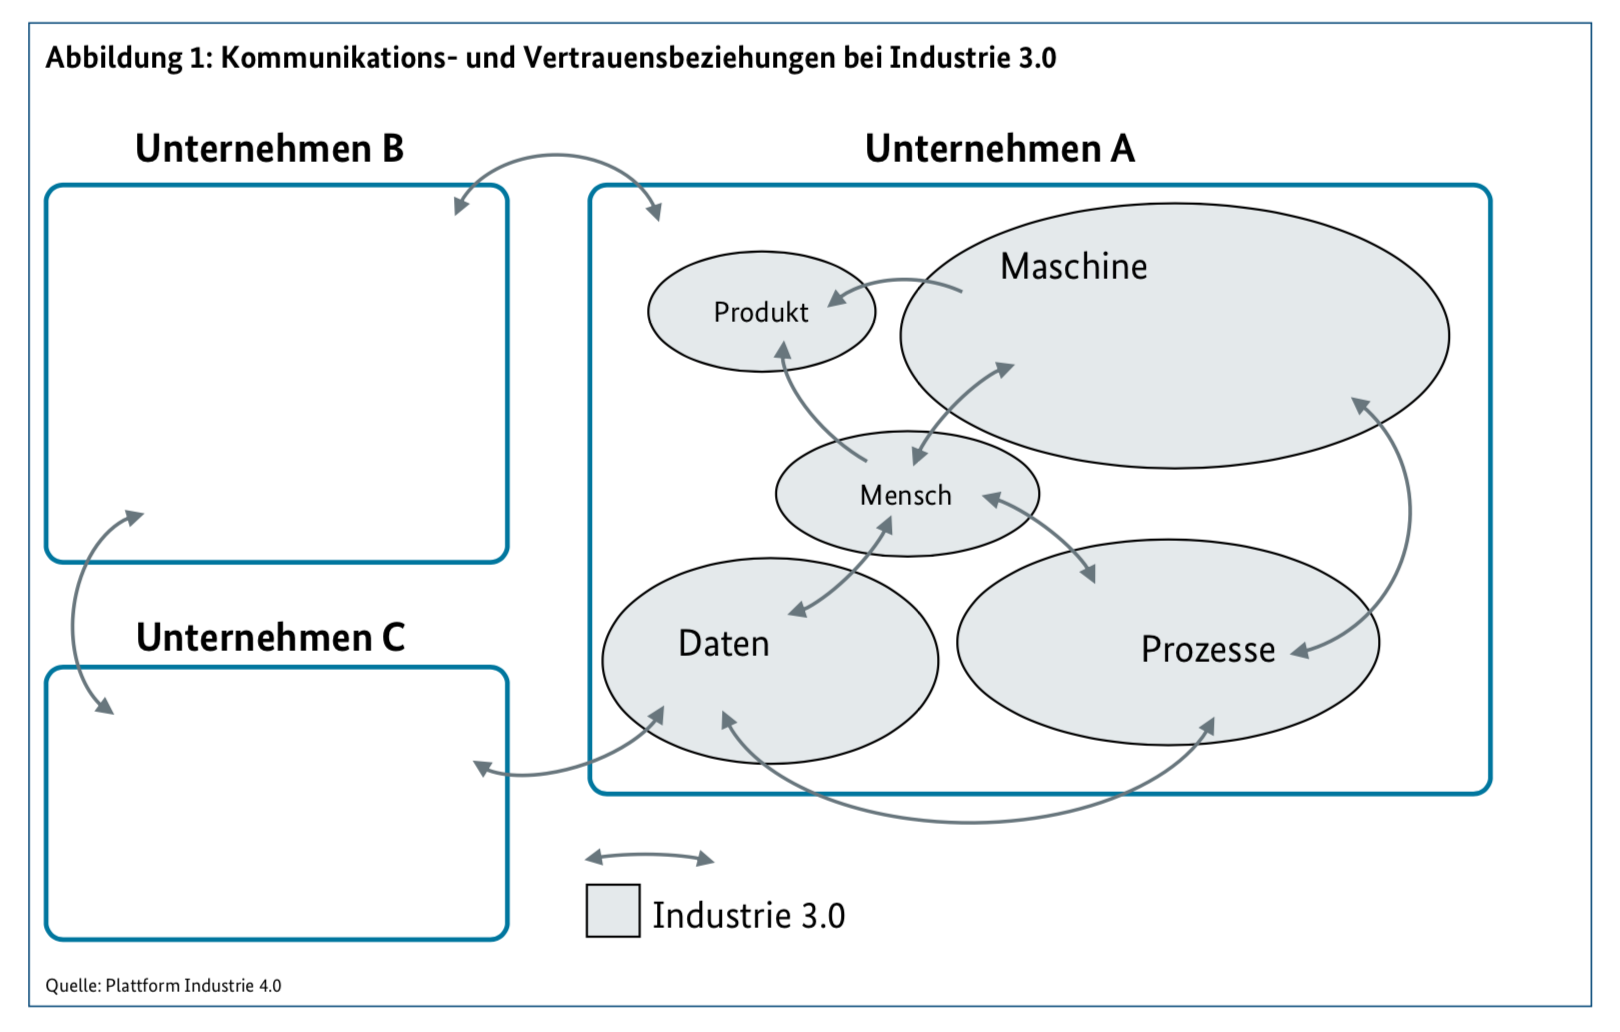
\includegraphics[width=15cm]{kommunikationsbeziehungen-i30}
  \caption{Kommunikationsbeziehungen in einer Industrie 3.0 Umgebung - TODO ref. sichere unternehmensübergreifende Kommunikation}
  \label{Kap2:Industrie3.0-Kommunikation}
\end{figure}

\clearpage

\subsection{4. industrielle Revolution}
Das Ende des 20. Jahrhunderts gilt als der Beginn der 4. industriellen Revolution. Das Kennzeichen dieser Phase ist die zunehmende Digitalisierung. Mit ihr geht die technische Vernetzung physischer Gegenstände, dem \ac{IoT}, einher. Mehr und mehr Geräte oder Gegenstände besitzen die Möglichkeit aktiv durch Datenaustausch oder passiv z. B. mit Hilfe eines Bar- oder QR-Codes mit der digitalen Welt zu kommunizieren und somit eine fortschreitende Automatisierung sowie Individualisierung zu ermöglichen. 

Im Gegensatz zur Industrie 3.0 sollen Maschinen autonom, auch über Unternehmensgrenzen hinweg, miteinander kommunizieren können um gesamte Geschäftsprozesse zu übernehmen. Dies setzt eine Öffnung der Unternehmen nach außen voraus.

\begin{figure}[h]
  \centering
  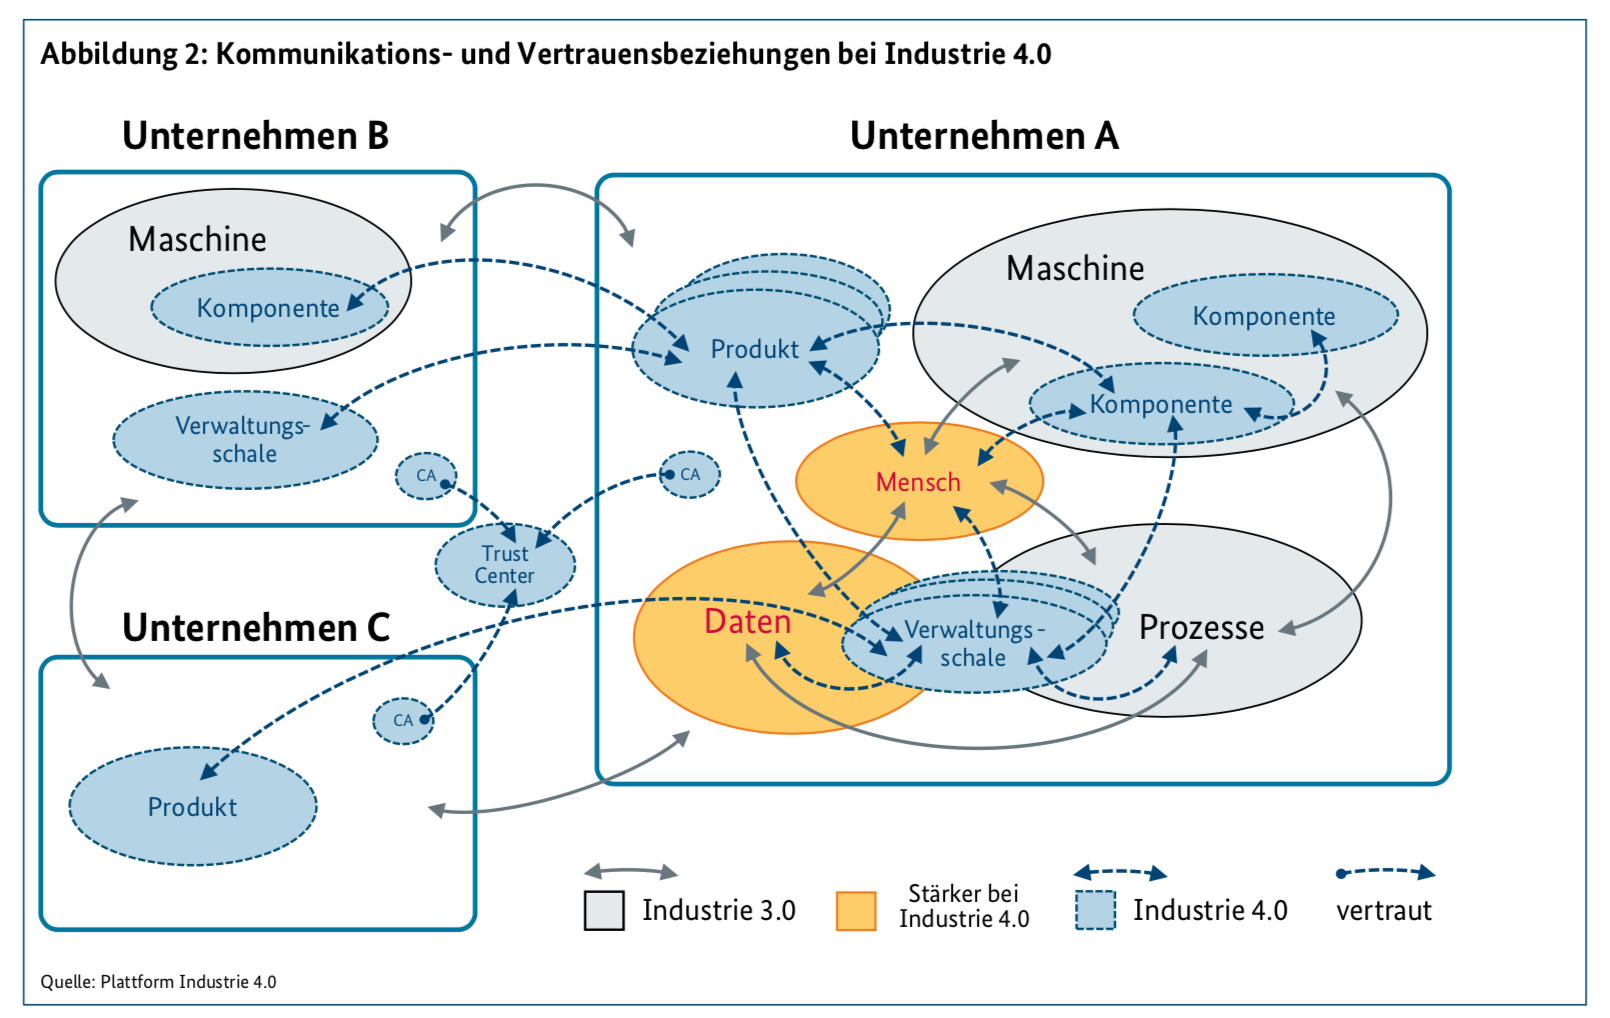
\includegraphics[width=15cm]{kommunikationsbeziehungen-i40}
  \caption{Kommunikationsbeziehungen in einer Industrie 4.0 Umgebung - TODO ref. sichere Unternehmensübergreifende Kommunikation}
  \label{Kap2:Industrie4.0-Kommunikation}
\end{figure}

\clearpage

Diese Entwicklung erzeugt durch die ständige Kommunikation eine ernome Menge an Daten, welche den Anforderungen der IT-Sicherheit gerecht werden müssen, um Verbraucher und Unternehmen zu schützen.

\section{aktueller Stand der Technik}
Der Prozess der vierten industriellen Revolution ist ein stetiger, nicht abgeschlossener Prozess. Aktuell werden die ersten Smart Factories der Industrie errichtet und erste smarte Einkaufsmöglichkeiten, wie Amazon Go und TODO - siehe Trumpf, für den Endverbraucher geschaffen. Diese Fabriken und Filialen stellen die ersten ihrer Art dar und dienen als Prototypen. Das Ziel des Wandels in der Strukturierung und Organisation der Produktion in Unternehmen ist eine immer weitere Automatisierung der Prozessabwicklung bis hin zu autonom arbeitenden Fabriken. Für kritische Infrastrukturen, wie z. B. im Energie-, Wasser-, Transport- und Gesundheitssektor existiert diese Verbindung bereits.

Die Umsetzung dieser Innovationen basiert hauptsächlich auf dem Fortschritt der \ac{IT} und dem Einzug der Internet-Technologien in die Industrie. Diese Entwicklung macht es möglich immer schneller Informationen auszutauschen, größere Datenmengen zu analysieren und diese zu verarbeiten. In der Industrie entstehen dadurch u. a. die folgenden Chancen:

\begin{itemize}
  \item Die Kommunikationsinfrastruktur wird in Zukunft in Produktionssystemen so preiswert sein, dass sie sinnvoll für Konfiguration, Service, Diagnose, Bedienung und Wartung genutzt werden kann.
  \item Die Produktionssysteme werden mehr und mehr mit einem Netz verbunden, erhalten dort eine digitale Identität, werden somit such- und analysierbar und besitzen die Möglichkeit Daten über sich selbst zu veröffentlichen. 
  \item Maschinen und Anlagen speichern ihre Zustände in ihrer digitalen Identität im Netz. Diese Zustände sind aktuell, aktualisierbar und zunehmend vollständig. Sind im Netzwerk viele solcher Identitäten vorhanden, können die Daten effizient abgerufen und ausgetauscht werden.
  \item Softwaredienste werden über das Netz verknüpft werden und können somit automatisiert individuelle Aufgaben durch die direkte Kommunikation der Systeme erledigen. Eine solche individuelle Wertschöpfung war bisher nur unwirtschaftlich oder gar nicht möglich.
\end{itemize}

Diese Veränderungen im Wertschöpfungsprozess und die ständige Kommunikation der Systeme bereiten jedoch auch Probleme. Es entstehen große Mengen an Daten, welche u. a. über einen unsicheren Kanal verbreitet werden sollen. Des weiteren sind viele vorhandene Produktionsanlagen nicht für diese Form von vermaschter Kommunikation entwickelt worden. Diesen Problemen wird aktuell durch die Entwicklung von Industriestandards und \ac{M2M}-Protokollen, wie z. B. die \ac{OPC UA} entgegengewirkt. Um vorhandene Anlagen weiterhin nutzen zu können, werden Gateways genutzt. (TODO Trumpf ref.)

\section{Industrie 4.0}
Der Begriff Industrie 4.0 wurde erstmals auf der Hannover Messe 2011 verwendet (\cite{drath2014}) und soll das Ergebnis der 4. industriellen Revolution darstellen. Der Grundgedanke hinter Industrie 4.0 ist die flächendeckende Vernetzung von Informations- und Kommunikationstechnik zu einem Internet der Dinge, Dienste und Daten (\cite{Spath2013}). Diese Vernetzung soll einen ständigen Informationsaustausch zwischen den Komponenten ermöglichen. Jede Komponente des \ac{IoT} soll als \ac{CPS} arbeiten. Ein \ac{CPS} besitzt neben seiner realen Identität eine digitale Identität, über welche es ständig mit anderen \ac{IoT}-Geräten kommunizieren kann. Kunden- und Maschinendaten werden miteinander vernetzt \cite{rami2016}.

\begin{figure}[h]
  \centering
  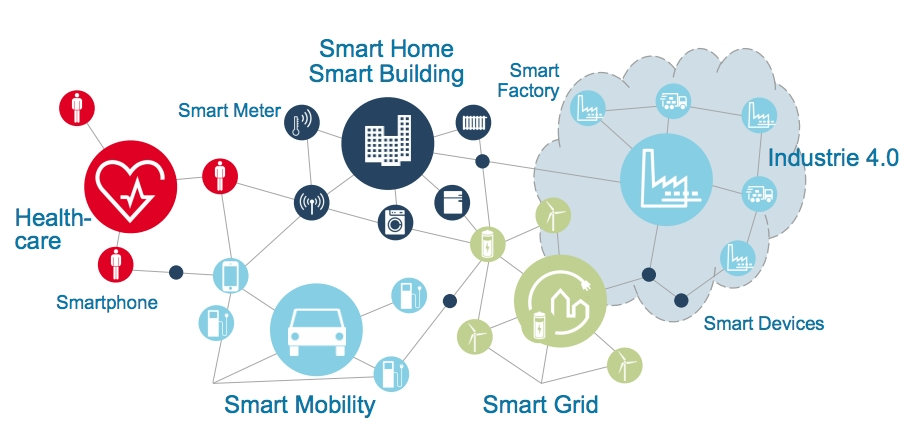
\includegraphics[width=15cm]{internet-der-dinge}
  \caption{Das Internet der Dinge - \cite{rami2016}}
  \label{Kap2:Das Internet der Dinge}
\end{figure}

\clearpage

Für Unternehmen bedeutet dies einen Wechsel von einer linearen Prozesskette hin zu einem vermaschten Netzwerk, in dem jede Komponente mit dem gesamten Netzwerk kommunizieren kann. Dies beinhaltet die Vernetzung der Komponenten auf horizontaler und vertikaler Ebene. Die vertikale Ebene stellt die technischen Komponenten dar und wird durch die Automatisierungspyramide beschrieben. Die horizontale Ebene beschreibt die wirtschaftlichen Geschäfts- bzw. Produktionsprozesse und besteht u. a. aus: Einkauf, Lieferanten, Produktionsplanung, Logistik, Sequenzierung und Lagerverwaltung. Das Ziel ist die Vernetzung aller Beteiligten.

\begin{figure}[h]
  \centering
  \includegraphics[width=15cm]{horizontaleVertikaleIntegration}
  \caption{horizontale und vertikale Integration - TODO ref. HP Industry-of-things siehe bookmark}
  \label{Kap2:horizontale und vertikale Integration}
\end{figure}

\clearpage

\subsection{\ac{IoT}/\ac{IIoT}}
\ac{IoT} beschreibt ein verbraucherorientiertes Konzept für die Nutzung von digitalisierten und vernetzten Systemen. Hierbei werden die physischen Systeme virtuell abgebildet. Dies wird genutzt, um die Effektivität der Systeme zu verbessern und intelligente Services zu nutzen. Das \ac{IIoT} beschreibt den Gebrauch von \ac{IoT}-Technologien im industriellen Raum.

Das \ac{IoT} ist ein wesentlicher Bestandteil der Industrie 4.0, welche Netzwerke aus Systemen, Daten und Dienstleistungen herstellt, in denen diese Komponenten miteinander kommunizieren. Für die Kommunikation haben sich, je nach Anforderungen, verschiedene Protokolle, wie z.B. \ac{HTTP}, \ac{CoAP}, \ac{XMPP} und \ac{MQTT}, etabliert. Jedes dieser Protokolle besitzt für spezifische Anforderungen wie Skalierbarkeit, vorhandene Ressourcen, Echtzeitkommunikation oder Sicherheit Vor- und Nachteile. 

\subsection{Automatisierungspyramide}
Die Automatisierungspyramide stellt die beteiligten Systeme und Softwarekomponenten eines automatisierten Prozesses systematisch dar. Diese beginnen, ausgehend vom Kundenauftrag und der betriebswirtschaftlichen Planung der Produktion auf der Unternehmensebene im \ac{ERP} System. Die Ergebnisse der Planung werden an das \ac{MES} übergeben, welches die verschiedenen Fertigungs- oder Logistikaufträge generiert. Die Aufträge werden anschließend auf der Prozessleit- (\ac{SCADA}), Steuerungs- (\ac{SPS}) und Feldebene (Ein-/Ausgangssignale) bearbeitet.

\begin{figure}[h]
  \centering
  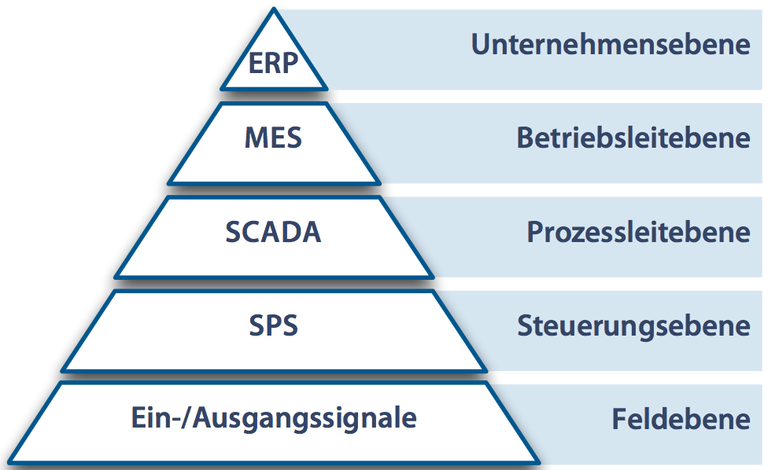
\includegraphics[width=10cm]{automatisierungspyramide}
  \caption{Automatisierungspyramide - TODO ref. Langmann,2004}
  \label{Kap2:Automatisierungspyramide}
\end{figure}

\clearpage

Während die oberen Schichten der Pyramide (\ac{ERP} und \ac{MES}) durch Standardkomponenten bzw. -software der IT realisiert werden, zählen die unteren Schichten (Prozessleit- bis Feldebene) zur Automatisierung, welche die Steuerung und Kontrolle der technischen Anlagen übernimmt. Diese werden auch als Shop-Floor-Ebene bezeichnet. Sie sind durch spezielle Hard- und Softwarelösungen umgesetzt. Die Kommunikation dieser Systeme ist u. a. für spezielle Anwendungsfälle wie harte Echtzeitkommunikation mit Verzögerungen <1ms ausgelegt. Die Integration von Sicherheitsmaßnahmen bei der Kommunikation dieser Systeme stellt oft eine große Herausforderung dar.

\section{Grundprinzipien der sicheren Kommunikation}
Die Grundprinzipien der sicheren Kommunikation beschreiben die Schutzziele im Bereich der Informationssicherheit. Diese verdeutlichen den Anspruch an die Sicherheit an ein zu implementierendes System oder ein Netzwerk. Sie stellen einen vereinbarten Umfang gegen Bedrohungen dar, welcher von den Kommunikationspartnern gewährleistet wird und nachgewiesen werden kann. Diese klassischen Schutzziele sind auch für Industrie 4.0 Umgebungen zutreffend. Die weitreichende Vernetzung der Systeme in der Industrie 4.0 erfordert jedoch weitere Schutzziele, um einen rechtskonformen Umgang oder besondere Anforderungen sicherzustellen.

\subsection{klassische Schutzziele}
\begin{itemize}
  \item Vertraulichkeit/Zugriffsschutz
  \item (Daten)-Integrität/Änderungsschutz
  \item Authentizität/Fälschungsschutz
  \item Verfügbarkeit
\end{itemize}

\subsection{weitere Schutzziele}
\begin{itemize}
  \item Verbindlichkeit/Nichtabstreitbarkeit
  \item Anonymität
\end{itemize}

TODO - gefällt mir nicht. Muss man die Begriffe erklären?
TODO - ref. \cite{BMWiSec2016}

\section{Kommunikationsstrukturen in Industrie 4.0 Umgebungen}
Um die Kommunikation zwischen verschiedenen Teilnehmern zu ermöglichen, ergeben sich in der Praxis unterschiedliche Strukturen. Jede dieser Strukturen bietet, je nach Anwendungsfall und zu erfüllenden Anforderungen, Vor- und Nachteile.

TODO - mehr -> siehe sichere Kommunikation-i4.0

\subsection{End2End}
Die Komponenten der Industrie 4.0 Umgebung kommunizieren über einen direkten Kanal miteinander. Dies setzt voraus, dass sich beide Teilnehmer in einem Netzwerk befinden, welches die benötigten Dienste wie z. B. \ac{IP} und \ac{DNS} zur Kommunikation bereitstellt. Des weiteren müssen beide Systeme diese Dienste und Protokolle unterstützen.

\subsection{Gateways}
Um existierende Systeme, welche selbst nicht Industrie 4.0 konform kommunizieren oder zu wenig Rechenleistung besitzen, in die Industrie 4.0 Welt zu integrieren, werden Industrie 4.0 Gateways genutzt. Dabei ist jedoch zu beachten, dass die Systeme hinter den Gateways nicht als Industrie 4.0 Komponenten entwickelt wurden und somit auch keine oder nur wenige dieser Eigenschaften besitzen. Des Weiteren ist es möglich, dass die Kommunikation aus Leistungsgründen oder besonderer Anforderungen über optimierte, proprietäre Protokolle stattfindet. Die Gateways müssen auf die Systeme und deren Protokolle individuell konfiguriert werden, um die Funktionalitäten im Industrie 4.0 Netz bereitstellen zu können, und die Kommunikation zu schützen.

\subsection{Publish-Subscribe}
Das Publish-Subscribe Modell bietet die Möglichkeit Informationen an mehrere Teilnehmer zu verteilen. Hierbei melden sich die Empfänger beim Verteiler an und wählen aus, über welche Nachrichtentypen sie informiert werden möchten. Diese Verteildienste nutzen zur besseren Skalierung und Reduzierung der Netzlast häufig Datagramme wie \ac{UDP}. Durch die Nutzung von Datagrammen geht jedoch die Fehlertoleranz verloren. Somit muss entweder dafür gesorgt werden, dass eine sehr zuverlässige Netzwerkinfrastruktur vorhanden ist und hohe Bandbreitenreserven geschaffen werden, um die Dienstgüte (\ac{QoS}) sicherzustellen oder dieses Modell nur für fehlertolerante Kommunikation wie z. B. Audio- und Video-Anwendungen oder Businessprozesse zu nutzen. 

\subsection{Kommunikation mit Netzwerk als Partner}
Zeitkritische Automatisierungsanwendungen verlangen besondere Netzwerkeigenschaften. Sie können auf Latenz oder Jitter angewiesen sein. Um diese Eigenschaften sicherzustellen, ist es sinnvoll in diese Netze eine Industrie 4.0 Schnittstelle zu integrieren. Somit ist es den Teilnehmern möglich, über die Verwaltungsschale sicherzustellen, dass das Netzwerk die erforderlichen Anforderungen bereitstellt. \cite{sichKom2017}

TODO - Bilder -> sichere-kommunikation-i40

\section{Normen und Standards}
Im Gegensatz zur Industrie 3.0, in welcher Daten auf lokaler Ebene oder zwischen einzelnen internen Unternehmensebenen ausgetauscht wurden, stellt der Datenaustausch und Informationsfluss im vermaschten Industrie 4.0 Netzwerk einen wesentlichen Bestandteil dar. Aktuell gibt es zwei Architekturmodelle zur Umsetzung von Industrie 4.0 Umgebungen. Diese setzen sich aus dem von der Platform Industrie 4.0 entwickelten \ac{RAMI4.0} und der \ac{IIRA} der \ac{IIC} zusammen. Beide Modelle verfolgen verschiedene Integrationsansätze.

Des Weiteren findet die Kommunikation in der Industrie 4.0 nicht mehr über einzelne, vorgegebene Schnittstellen statt, sondern direkt von den Produktionssystemen, also den unteren Ebenen der Automatisierungspyramide. Um dies zu ermöglichen, ist es notwendig, eine einheitliche Kommunikation durch Normen und Standards herzustellen, um eine unternehmensübergreifende Kommunikation dieser Shop-Floor IT zu ermöglichen. 

\subsection{TCP/IP Referenzmodell}
Das TCP/IP Referenzmodell ist ein Schichtenmodell, welches die vier Schichten der Internetprotokollfamilie beschreibt. Sie setzen sich aus Application-, Transport-, Internet- und Link-Layer zusammen. Die Schichten des TCP/IP Referenzmodells überlagern sich mit den Schichten des ISO/OSI Referenzmodells.

\subsubsection{Application Layer}
Die Anwendungsschicht ist für die Übertragung der Nutzdaten zwischen verschiedenen Anwendungen zuständig. Dabei kann es sich um entfernte Anwendungen handeln. Diese sollen sich für den Benutzer verhalten, als würden sie lokal ausgeführt werden.

TODO - Prozess- und Businesslogik

\subsubsection{Transport Layer}
Die Transportschicht sorgt für die Kommunikation zwischen Prozessen. Die Transportschicht nutzt Ports um verschiedene Dienste zu adressieren. Sie beeinflusst, ob es sich um eine zuverlässige Verbindung ( TCP ) oder nicht ( UDP ) handelt.

TODO - End2End Security

\subsubsection{Internet Layer}
Die Internetschicht wird genutzt, um Daten von einem Teilnehmer im Netzwerk zum anderen zu übertragen. Die Endpunkte im Netzwerk werden durch IP Adressen beschrieben.

\subsubsection{Link Layer}
Der Bitübertragungsschicht beschreibt die Topologie des Netzwerks. Sie stellt die physikalische Verbindung der Netzwerkteilnehmer zur Verfügung.

TODO - Bild Interenetprotokollfamilie

\subsection{Industrie 4.0 Referenzarchitekturen}
\subsubsection{\ac{RAMI4.0}}
Um eine flächendeckende Vernetzung zu ermöglichen, muss eine einheitliche Kommunikation geschaffen werden. Die \ac{RAMI4.0} ist eine dreidimensionale Darstellung aller Teilnehmer einer Industrie 4.0 Umgebung und stellt ein Modell einer \ac{SOA} dar. Sie soll eine Verwaltungsschale für Teilnehmer bilden, um eine standardisierte Kommunikation und einfache Inbetriebnahme neuer Komponenten ermöglichen. \cite{rami2016} Die Achsen des \ac{RAMI4.0} bestehen aus:

\begin{itemize}
  \item Achse 1 - Die Hierarchie zeigt die Anlagen, Maschinen sowie das Endprodukt, welche miteinander Vernetzt sind. In diesem Netzwerk werden Funktionen bereitgestellt und Daten ausgetauscht.
  \item Achse 2 - Die Architektur beschreibt - TODO
  \item Achse 3 - Der Produktlebenszyklus wird im Gegensatz zur Industrie 3.0 in das Netzwerk mit eingebunden. Der gesamte Prozess der Produktion, Wartung bis hin zur Verschrottung soll digital erfasst werden.
\end{itemize}

\begin{figure}[h]
  \centering
  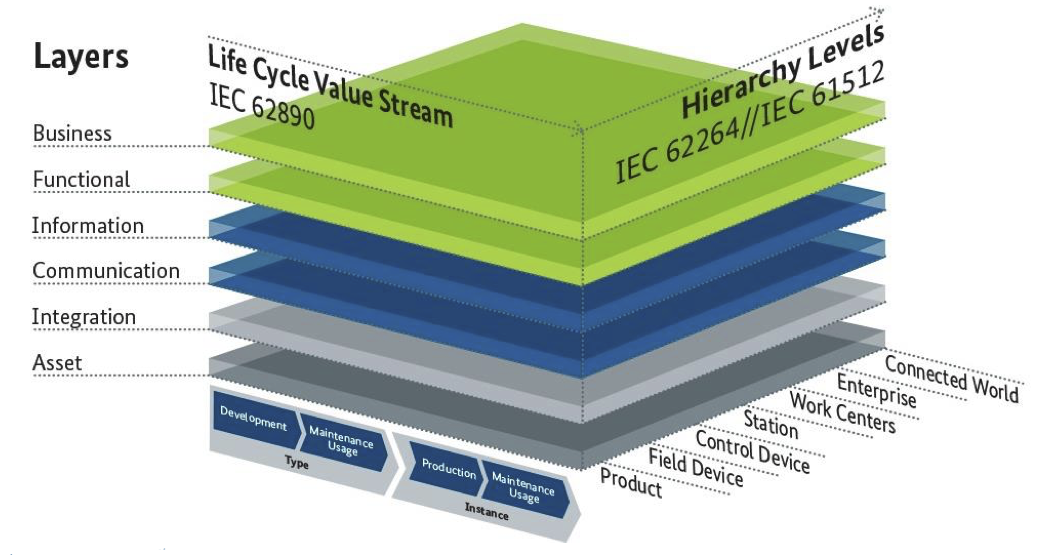
\includegraphics[width=15cm]{rami40}
  \caption{RAMI 4.0 - \cite{rami2016}}
  \label{Kap2:RAMI 4.0}
\end{figure}

\clearpage

Nach dem \ac{RAMI4.0} stellt der Communication Layer das Bindeglied zwischen dem Integration Layer, welcher Eigenschaften der physischen Welt für Computersysteme erreichbar macht, und dem Information Layer, welcher die Funktionsbezogenen Daten beinhaltet, dar. \cite{BMWiNeCon2016} 

TODO - Kommunikation beschreiben

Jeder Teilnehmer der Architektur wird als Asset bezeichnet und besitzt seine eigene Verwaltungsschale, welche als Schnittstelle zum Austausch von Informationen dient. Die Verwaltungsschale ist der Übergang zwischen der physischen zur digitalen Welt.

TODO - genauer auf die einzelnen Komponenten eingehen! - Assets, Architektur, Komponenten, Verwaltungsschale
TODO - Architektur wichtig SOA beschreiben -> Angriffsvektoren
TODO - siehe DIN 91345
TODO - Anforderungen an diese Komponenten unterschiedlich

\subsubsection{IIRA}
TODO

\subsection{Protokollstandards}
TODO - Durch die vorausgesetzte M2M-Kommunikation wurde die Entwicklung neuer Protokolle zum effizienten Informationsaustausch vorangetrieben, welche es ermöglichen sollen, eine Standardisierung bereitzustellen und somit eine herstellerübergreifende und plattformunabhängige Kommunikation zu ermöglichen.

\subsubsection{OPC UA}
TODO

\subsubsection{DDS}
TODO

\section{Testsystem}
Die aus der Analyse hervorgehenden möglichen Schwachstellen im Bereich der Netzwerksicherheit und deren Auswirkungen werden anhand eines vorhandenen, prototypischen Industrie 4.0 Testsystems \cite{Weber2018} veranschaulicht. Das vorhandene System setzt die drei Schichten der Software-Architektur (Verteilungs-, Baustein- und Laufzeitschicht) nach Starke / Hruschka um. Die Netzwekkommunikation wird über das Protokoll OPC UA realisiert, welches die Anforderungen der Industrie 4.0 und \ac{RAMI4.0} umsetzt.

\subsection{Architektur}
Das vorhandene System ist, aufgrund der vorgesehenen Einsatzgebiete Lehre, Integrations- und Sicherheitstests, als \ac{VM} umgesetzt worden. Dies ermöglicht es die Testinfrastruktur vom restlichen Netz zu kapseln. Das Betriebssystem der \ac{VM} stellt eine Firewall bereit, welche unerwünschten Netzwerktraffic von oder zu dem System verhindert. Um eine gute Erweiterbarkeit der Testumgebung und Modularisierung der Komponenten zu erreichen, werden die einzelnen Industrie 4.0 Komponenten mit Hilfe der Containerlösung Docker isoliert ausgeführt, verwaltet und deren Netzwerkkommunikation sichergestellt. Durch den zusätzlichen Einsatz des Deploymentsystems Kubernetes wird ein verteiltes Ausführen des Systems ermöglicht und somit eine gute Skalierbarkeit erreicht. 

\subsection{Komponenten}

\subsubsection{Repository}
\subsubsection{Discovery Server}
\subsubsection{\ac{PKI}}
\subsubsection{Identity Provider}
\subsubsection{Verwaltungsinterface}
\subsubsection{Scheduler}
\chapter{Konzept}
TODO - Konzept komplett überarbeiten. Siehe 1. Absatz Analyse z.B.

Um die in den Grundlagen beschriebenen Sicherheitsstandards, Protokolle und Integrationslösungen auf ihre Standhaftigkeit in Bezug auf die IT-Schutzziele zu analysieren, werden die Protokolle und Systeme in ihrem Aufbau untersucht und mögliche Schwachstellen herausgearbeitet, daraus hervorgehende Risiken beschrieben und erforderliche Maßnahmen empfohlen. Die \ac{RAMI4.0} beschreibt ein Referenzmodell für Industrie 4.0 Umgebungen. Bereits etablierte Lösungen bestehen aus heterogenen, individuellen Netzwerklandschaften. Um eine Untersuchung der vorhandenen Systeme im neuen Umfeld durchzuführen, müssen verschiedene Faktoren, wie Infrastruktur oder besondere Anforderungen an die Systeme mit einbezogen werden. Das folgende Kapitel dient der Beschreibung der Vorgehensweise bei der Analyse der Netzwerkkommunikation und deren Komponenten.

\section{Komponenten}
Die beschriebenen Anforderungen müssen, um eine sichere Netzwerkkommunikation zu gewährleisten, von allen beteiligen Komponenten der Umgebung integriert und umgesetzt werden. Industrie 4.0 Umgebungen können in unterschiedlichster Form ausgeprägt sein. Die Umsetzung der Hard- und Softwarekomponenten hängt von den zu übertragenden Daten, dem Übertragungsmedium, der Übertragungsdistanz und vorausgesetzten Dienstgüte ab. Die zu analysierenden Komponenten werden in Hard- und Softwarekomponenten gegliedert.

\subsection{Hardware}

TODO

\subsubsection{Übertragungskanal}
Der Übertragungskanal beschreibt die Bitübertragungsschicht. In Industrie 4.0 Umgebungen ist es notwendig, Daten zu übertragen, um eine räumliche oder zeitliche Distanz zu überbrücken. Je nach Anwendungsfall findet diese Kommunikation über Kupfer- bzw. Glasfaserkabel, Funkübertragung oder ein Speichermedium statt. Je nach Beschaffenheit des Übertragungskanals, ist es notwendig, weitere Maßnahmen zur Sicherheit der Kommunikation zu treffen. Aufgrund der Durchführung der Analyse in einem virtuellen Testsystem, werden die Auswirkungen der Form des Übertragungskanals bei der Analyse der Kommunikation nicht beachtet.

\subsection{Software}
Jede Komponente einer \ac{ICS}-Umgebung kann Softwareschwachstellen und Sicherheitslücken enthalten. Dabei spielt es keine Rolle, ob es sich um ein komplexes \ac{ICS} handelt oder um einen einfachen Anwendungsserver. Software-Aktualisierungen sowie ein Patch-Management sind für einen sicheren Betrieb notwendig, um Angriffe über Exploits zu verhindern. 

\subsubsection{Netzwerkstack}
Die Kommunikation zwischen Industrieanlagen findet mehr und mehr auf der Basis von TCP-basierten Netzwerken statt. Das \ac{RAMI4.0} beschreibt Industrie 4.0 Umgebungen als \ac{SOA}. \ac{SOA} beschreibt ein Netzwerk, in welchem von den Teilnehmern Dienste bereitgestellt und genutzt werden können. Die Dienste im Netzwerk werden i. d. R. über eine \ac{REST}-\ac{API} bereitgestellt. Diese Schnittstellen nutzen bereits etablierte Protokolle der \ac{IoT} oder \ac{IIoT} Welt.

\subsubsection{Protokolle}
\ac{IoT}-Geräte nutzen das Internet als Übertragungsmedium. Somit müssen sie zur Übertragung ihrer Daten Protokolle nutzen, welche die Internet Protocol Suite der \ac{IETF} einhalten. Etablierte Internet-Protokolle wie HTTP und XMPP wurden zur Kommunikation ressourcenreicher Geräte mit hoher Leistung entwickelt und sind für viele Netzwerke mit \ac{IoT}- oder \ac{IIoT}-Endknoten zu komplex, bzw. nicht geeignet. Im Rahmen der 4. industriellen Revolution wurden daher, vor allem für \ac{IIoT} Umgebungen, neue Protokolle entwickelt, welche ressourcensparende, sichere Kommunikation zwischen Maschinen bereitstellen sollen. 

TODO - CoAP, MQTT

\section{Abgrenzung}
Die \ac{IIRA} ist ein anerkannter, in der Industrie verbreiteter Standard. Da die Analyse der Netzwerksicherheit am in \autoref{Grundlagen:Testsystem} beschriebenen Testsystem durchgeführt werden soll, welches den Kommunikationsstandard \ac{OPC UA} implementiert, wird sich im weiteren Verlauf der Thesis ausschließlich auf die in der IEC 62541 beschriebene Architektur \ac{RAMI4.0} als Referenzmodell zur Analyse bezogen. Es werden Bedrohungen in Industrie 4.0 Umgebungen beschrieben, eine Analyse der Übertragungsmedien und Infrastruktur durchgeführt und die im Testsystem verwendeten Protokolle mit Bezug auf ihre Anforderungen im Bereich der Netzwerksicherheit untersucht. Um verschiedene Praxisszenarien darzustellen, wird das Testsystem um für die Analyse benötigte, zusätzliche Komponenten erweitert. 

\section{Vorgehensweise}
Die Analyse der Netzwerkkommunikation der unteren Schichten (Internet- und Link Layer) des im \autoref{Grundlagen:TCP/IP Referenzmodell} beschriebenen TCP/IP Referenzmodells wird auf Basis der in \autoref{Grundlagen:Grundprinzipien der sicheren Kommunikation} erläuterten Schutzziele durchgeführt. Die oberen Schichten (Transport- und Application Layer) werden in der Testumgebung durch das \ac{M2M}-Protokoll \ac{OPC UA} realisiert. Hierbei dient die Spezifikation des Protokolls als Grundlage der Analyse. Aus der Spezifikation ergeben sich die bei der Kommunikation für die IT-Sicherheit zuständigen Komponenten von \ac{OPC UA}. Diese werden nach des Anforderungen des TODO - ref. BSI ICS Security Kompendium und FIRST CVSS v2.0 - auf Sicherheitslücken und Widersprüche untersucht. Bei der Analyse auftretende, mögliche Schwachstellen werden in einer vorhandenen, prototypischen Industrie 4.0 Testumgebung \cite{Weber2018} implementiert und nachgewiesen. Sicherheitslücken, welche durch Fehlkonfiguration auftreten und keine konzeptionellen Schwachstellen der Software oder deren Protokolle darstellen, sollen in der Testumgebung aktiviert und deaktiviert werden können, um die Auswirkung eines Angriffs auf ein Industrie 4.0 System zu Lehr- und Testzwecken darstellen zu können.
\chapter{Analyse}
\section{Risiken}
Die vierte industrielle Revolution, das \ac{IIoT} und dessen Vielzahl an aktiven und passiven Elementen stellen in ihrer Komplexität eine große Herausforderung für die IT-Sicherheit dar. Einerseits muss die Sicherheit der laufenden Software, der Infrastruktur, Anwendungs- und Rechnersysteme gewährleistet werden, andererseits muss die Betriebssicherheit der Geräte und Anlagen, welche mit dem Internet verbunden sind sichergestellt werden. Das Management der IT-Sicherheit in Industrie 4.0 Netzen geht über Unternehmensgrenzen hinweg, da Netze und Systeme für Kunden, Lieferanden und Partner bereitgestellt werden \cite{DTAG2016}. Somit hat sich auch die Bedrohungslage der Netze geändert. Das \ac{BSI} beschreibt die Top 10 Bedrohungen und deren Folgen für \ac{ICS} \cite{ICSSec2016}.

\begin{enumerate}
    \item Social Engineering und Phishing - 
    \item Einschleusen von Schadsoftware über Wechseldatenträger und externe Hardware - 
    \item Infektion mit Schadsoftware über Internet und Intranet - 
    \item Einbruch über Fernwartungszugänge - 
    \item Menschliches Fehlverhalten und Sabotage - 
    \item Internet-verbundene Steuerungskomponenten - 
    \item Technisches Fehlverhalten und höhere Gewalt - 
    \item Kompromittierung von Extranet und Cloud Komponenten - 
    \item \ac{DoS} und \ac{DDoS} - 
    \item Kompromittierung von Smartphones im Produktionsumfeld - 
\end{enumerate}

TODO - ref. nach BSI
TODO - Bedrohungsanalyse

Um die in \autoref{Grundlagen:Grundprinzipien der sicheren Kommunikation} genannten Schutzziele umzusetzen, ist es notwendig einen größtmöglichen Schutz gegen diese Bedrohungen bereitzustellen. Dafür müssen die Netzwerkinfrastruktur, Integrationsansätze und die eigentliche Kommunikation über die genutzten Protokolle gesichert werden. Dies geschieht u.a. durch die Abschottung von Systemen, die Einschränkung von Zugangsberechtigungen, die Härtung der Sicherheit der genutzten Komponenten, den Einsatz von Verschlüsselungsverfahren und die Schulung der Mitarbeiter um ein Sicherheitsbewusstsein zu schaffen und die Einhaltung von Sicherheitsrichtlinien zu gewährleisten.

\section{Netzwerkinfrastruktur}
TODO - heterogene Netze machen Probleme - Globale Netze haben Latenz, Paketverlust, usw.; müssen Anforderungen gerecht werden.

\subsection{Übertragungsmedium}
Als Übertragungsmedien können neben der klassischen Kabelverbindung auch andere (instabile) Kanäle wie Mobilfunk oder Satelliten in Frage kommen. Um die Kommunikation über alle Medien sicher und zuverlässig zu gestalten, müssen auf technischer Ebene Protokolle genutzt werden, welche es ermöglichen die gegebenen Schutzziele zu realisieren und die Integrität der Daten bei der Übertragung über große Entfernungen zu gewährleisten.

TODO - Übertragungsdistanz - Latenz - Jitter - usw.

\subsection{Defense in Depth Strategie}
Die Norm IEC 62443 - TODO ref. - beschreibt ein Defense in Depth Konzept, um die IT-Sicherheit der Anlagen, die Netzwerksicherheit und Systemintegrität nach dem Stand der Technik zu schützen. Sie gliedert eine Unternehmensinfrastruktur in multiple und redundante Sicherheitsschichten (Zonen), um ein höchstmögliches Sicherheitsniveau zu erreichen. Die unabhängigen Verteidigungslinien sollen Angriffe verzögern, um Zeit für Gegenmaßnahmen zu gewinnen.

Die Kommunikation erfolgt in separierten Netzsegmenten, welche zusätzlich mit \ac{IDS} nutzen, um Angriffe schnell zu erfassen und Gegenmaßnahmen einleiten zu können. Somit wird der Aufwand, um die Shop-Floor-Ebene zu kompromittieren durch den Einsatz von \ac{DMZ}, \ac{IDS}, Paketfilter und Time Access Control wesentlich erhöht. Zusätzlich ist das "`Zone and Conduit"' Modell eines der zentralen Elemente der Defense in Depth Strategie. Die verschiedenen Zonen können nur mittels spezieller Leitungen (Conduits) miteinander kommunizieren.  

\begin{figure}[h]
    \centering
    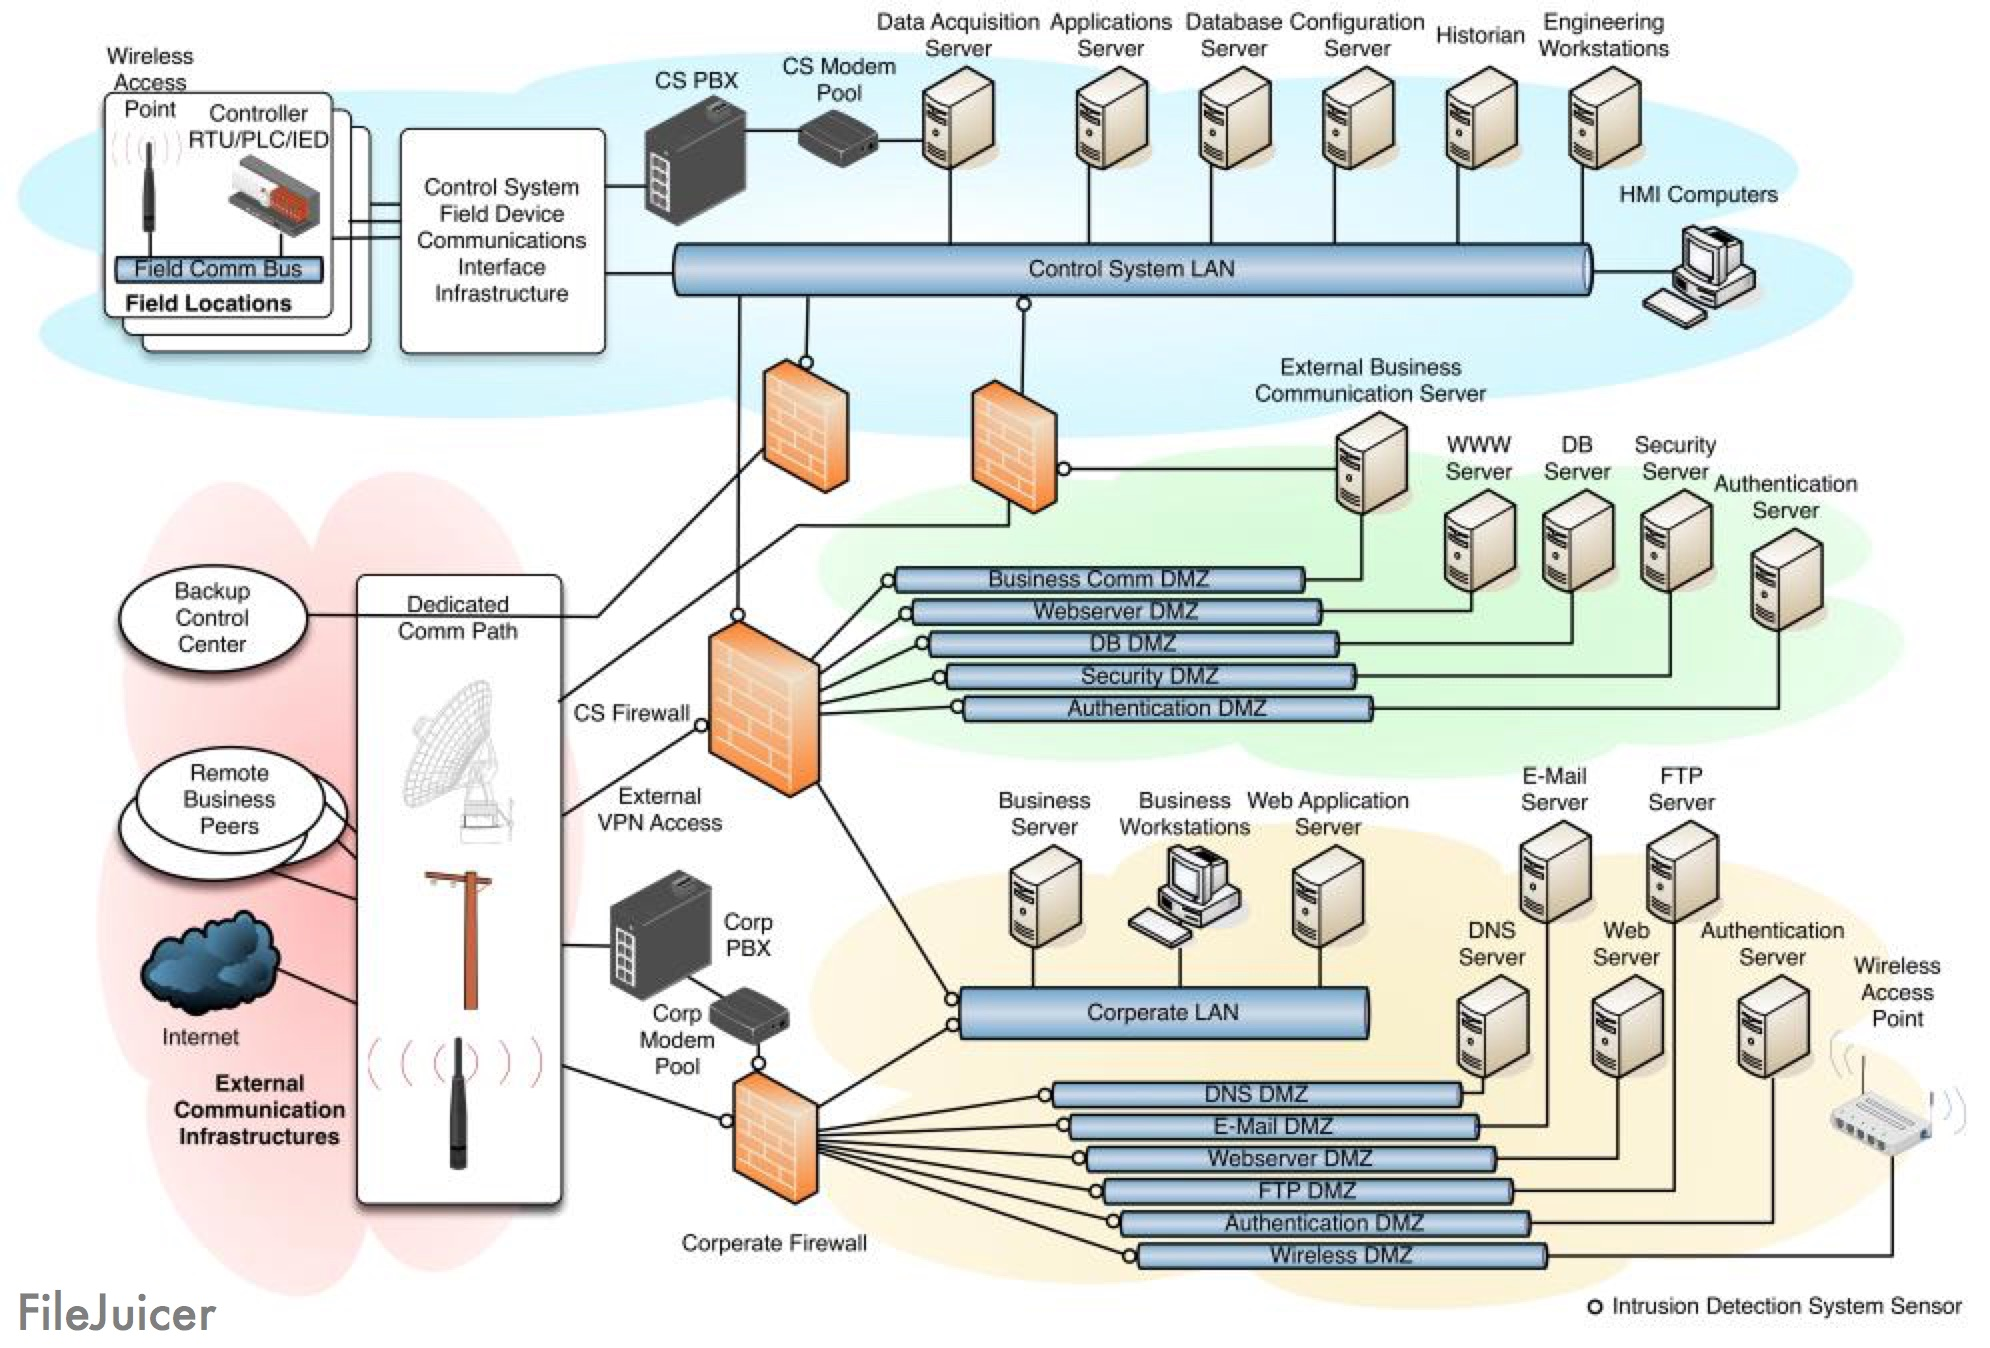
\includegraphics[width=15cm]{defense-in-depth-strategie}
    \caption{Defense in Depth Strategie - \cite{kuipers2006}}
    \label{Kap3:Defense-in-Depth}
\end{figure}

\clearpage

Das Defense in Depth Konzept stellt ein Konzept dar, um Industrieanlagen und Unternehmensnetzwerke vor Angriffen zu schützen. Bei der sich ständig ändernden Bedrohungslage in den komplexen Netzen wird bei dieser Strategie jedoch weniger ein vollständiger Schutz bereitgestellt, als eine Strategie zur Schadensbegrenzung im Falle eines Angriffs.

\section{Integrationsansätze}
Die Grundlage der Industrie 4.0 Kommunikation ist ein standardisierter Datenaustausch über alle Schichten der Automatisierungspyramide hinweg. Dabei stellt der \ac{IEC}-Standard \ac{OPC UA} einen vielversprechenden Ansatz für einen standardisierten Informationsaustausch über Unternehmensgrenzen hinweg dar. Jedoch müssen auch bestehende Systeme in die Industrie 4.0 Kommunikation integriert werden. Dies führt häufig zu Problemen, da diese Systeme proprietäre Protokolle nutzen, besondere Anforderungen wie Echtzeitkommunikation besitzen oder gar keine Schnittstelle bereitstellen. Es bestehen grundsätzlich zwei Ansätze zur Integration dieser Anlagen. TODO - ref.

\subsection{Konsolidierung der Netzwerkkommunikation}
TODO - Eine Möglichkeit der Entwicklung zu einer Smart Factory ist die Konsolidierung die Netzwerkkommunikation. Fokus auf OPC UA, da standardisiert.
TODO - neue Netze/Factories können so geplant werden, dass die Maschinen die benötigten Schnittstellen bereitstellen.
Ansatz: teuer, aufwendig bzw. nicht möglich, da embedded System bzw. keine Ressourcen oder keine Schnittstellen

\subsection{Gatewaykommunikation}
Eine Alternative zur Umstellung der bestehenden Systeme stellt die Kommunikation über Gateways dar. Hierbei gibt es mehrere Softwarelösungen, welche unterschiedliche Ziele verfolgen. Es werden Systeme zur Anlagenoptimierung (TODO - ref. SePiA.Pro), der Bereitstellung einer offenen, branchenübergreifenden Plattform mit diversen Smart Services wie Datenanalyse und Flottenmanagement (TODO - ref. Siemens Mindsphere, DeviceInsight) und dem herstellerübergreifenden Gerätemanagement (AXOOM) entwickelt \cite{acatec2016}. Die Systeme sammeln und verwalten die Daten der Anlagen an zentraler Stelle und stellen sie im Netzwerk zur Verfügung. Der Einsatzmöglichkeiten dieser Softwarelösungen sind von den vorhandenen Schnittstellen der Anlagen abhängig und benötigen eine individuelle Konfiguration um den unterschiedlichen Anforderungen der Industrielandschaft gerecht zu werden.

TODO - Im folgenden Abschnitt wird die Umsetzung der Kommunikation über eine digitale Serviceplattform am Beispiel von AXOOM dargestellt.

\subsubsection{AXOOM}
TODO - Gründe der Wahl von AXOOM: 
TODO - 2016 Innovationspreis deutsche Indsutrie
TODO - unterstützt Optimierung der Wertschöpfungskette -> ERP-, MES Kommunikation über "bekannte", offene Schnittstellen (REST usw.) 
TODO - unterstützt Anbindung von \ac{IoT}. Analyse und Visualisierung von Daten -> Kommunikation über spezielle Schnittstellen

\begin{figure}[h]
    \centering
    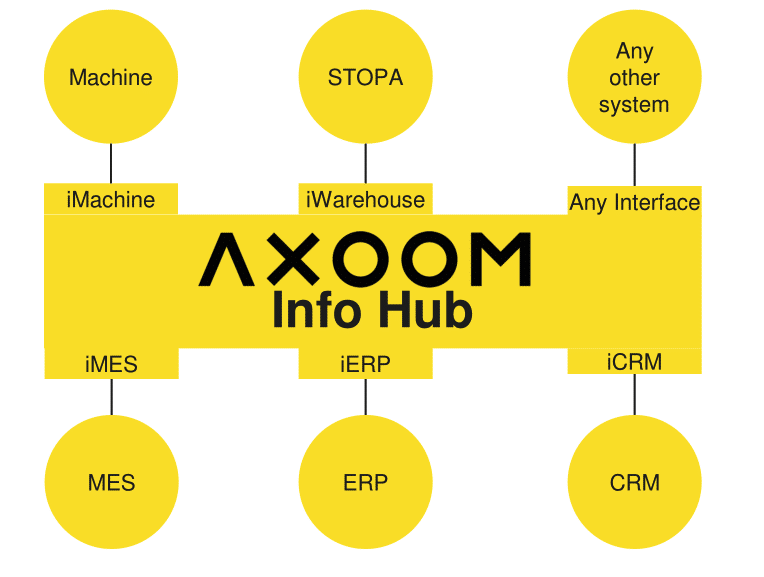
\includegraphics[width=15cm]{axoom-integration}
    \caption{AXOOM Netzwerkintegration}
    \label{Kap3:AXOOM Netzwerkintegration}
  \end{figure}
  
\clearpage

TODO - sichere Kommunikation durch AXOOM Gate - wie? Quellen? -> "Dieses basiert teilweise auf Technologien unseres Partners C-Labs und schafft eine direkte Verbindung zwischen dem Kundennetzwerk und der Cloud. Das AXOOM Gate ist in der Lage, Daten herstellerunabhängig von allen angebundenen Geräten zu sammeln, so dass diese verschlüsselt an die AXOOM Plattform gesendet und dort visualisiert und ausgewertet werden können. Besonderen Schutz bei der Datenübertragung bietet ein mehrstufiges Sicherheits- und Verschlüsselungskonzept auf Komponenten-, Transport-, Applikations- und Anwenderebene. So wird eine genaue Zugriffskontrolle innerhalb der Fabrik sowie auf die Fabrik sichergestellt, unsichere Verbindungen von und nach Außen sind ausgeschlossen."

\subsubsection{Schnittstellen}
TODO - offene Schnittstellen für Low Level
TODO - REST usw. für High Level Applications

\subsubsection{andere Kriterien}
TODO - Softwareschwachstellen, Softwarefehler 
TODO - Herstellerabhängigkeit
TODO - Kosten der Interfaceentwicklung, usw.

\section{\ac{OPC UA} Protokollanalyse}

TODO - The OPC UA specifications are layered to isolate the core design from the underlying computing technology and network transport. This allows OPC UA to be mapped to future technologies as necessary, without negating the basic design. Mappings and data encodings are described in Part 6. Three data encodings are defined:
\begin{itemize}
    \item XML/Text
    \item UA Binary
    \item JSON
\end{itemize}
In addition, several protocols are defined:
\begin{itemize}
    \item OPC UA TCP
    \item HTTPS
    \item WebSockets
\end{itemize}

TODO - ref. OPC Pt. 1

\subsection{Bedrohungsanalyse}
TODO - siehe BSI UPC UA Analyse.

\subsection{Darstellung der bzgl. IT-Sicherheit wichtigen Komponenten}


TODO - \ac{OPC UA} ist in der \ac{IEC} 62541 als offener Standard definiert und erstreckt sich über Communication- und Information Layer des \ac{RAMI4.0}, da es eine \ac{SOA} bereitstellt. 
TODO - vereint Daten und Informationsdienste. 
TODO - basiert auf IP-Netz -> Angriffsvektoren von IP und genutzten Diensten immer noch zutreffend

\begin{figure}[h]
    \centering
    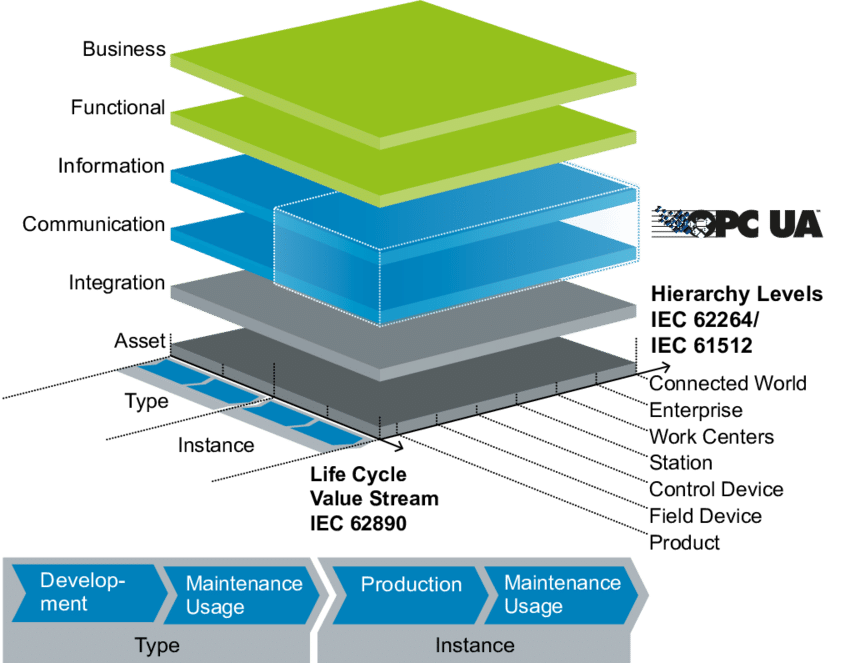
\includegraphics[width=15cm]{opcua_rami40}
    \caption{OPC UA im RAMI 4.0}
    \label{Kap3:OPC UA im RAMI 4.0}
  \end{figure}
  
\clearpage

\section{Angriffsvektoren}
\subsection{\ac{OPC UA} Spezifikation}
\subsubsection{Sicherheitslücken}
\subsubsection{Widersprüche}
\subsubsection{}

\subsection{Verschlüsselung}
\subsection{Paketversand}
\subsection{TODO}

\section{Auswertung der Ergebnisse}
\subsection{Probleme der Spezifikation}
TODO - Widersprüche in Spezifikation, sonstiges -> Syntaxfehler, usw.

\subsection{Erweiterung des Testsystems}
TODO - gefundene Schwachstellen bzw. Fehlkonfigurationen sind Grundlage der Implementierung!
\chapter{Validierung}
Mit der Implementierung und Durchführung der Angriffe wird das in (\autoref{Konzept}) erstellte Konzept validiert.
\chapter{Fazit}
Die Ziele der durchgeführten Arbeiten bestanden zum Einen aus der Analyse der Netzwerkkommunikation in Industrie 4.0 Netzen und zum Anderen aus der Erweiterung des Testsystems anhand der Ergebnisse der Analyse. Die Darstellung der Ergebnisse der Analyse durch verschiedene Anwendungsszenarien war mit Hilfe des vorhandenen Softwarestacks im Testsystem nur  begrenzt möglich. Um das Angriffsszenario eines \ac{MitM} Angriffs mit Hilfe eines Rogue \ac{DHCP} Servers darstellen zu können, wurde die Netzwerkkommunikation der in den Ergebnissen dargestellten Komponenten durch die Virtualisierung von zwei Netzwerken umgesetzt. Die Netzwerke beinhalten zwei weitere \ac{VM}s welche die verschiedenen Komponenten des Netzwerks repräsentieren. Diese bestehen aus \ac{DHCP}, \ac{DNS}, \ac{CoAP} Client und Server sowie Maniplations- und Monitoringsystem. Der \ac{DHCP} stellt die Netzwerkkonfiguration bereit und ermöglicht den Betrieb der weiteren Komponenten. Durch die eigene Verwaltung des \ac{DNS} Servers ist es in Zukunft möglich weitere Anwendungsszenarien am Testsystem darzustellen. Dazu gehören u. A. der in \autoref{Analyse:DNS Amplification} beschriebene Angriff der \ac{DNS} Amplification durch die Generierung eigener Zonen mit extrem vielen \ac{RR}, um eine möglichst große \ac{DNS} Response zu provozieren sowie das \ac{DNS} Spoofing und die Analyse der Sicherheitsmechanismen von \ac{DNSSEC}. Die \ac{CoAP} Komponenten werden zur Durchführung und Visualisierung der Kommunikation im Netzwerk genutzt.

Die Angriffsszenarien sowie die Änderungen am Testsystem wurden zuerst konzipiert und anschließend durchgeführt. Die Erweiterung des Testsystems nimmt, mit Ausnahme der Implementierung eines Verschlüsselungsverfahrens während dem Nachrichtenaustausch der Komponenten, keinen Einfluss auf den bisher implementierten Produktionsprozess und dessen Containervirtualisierung. 

Die Skalierbarkeit des Testsystems bleibt hinsichtlich weiterer dargestellter Komponenten und Prozesse durch das Protokoll \ac{OPC UA} sowie der Erweiterung des virtuellen Netzwerks um weitere \ac{VM}s und zur Analyse neuer Technologien erhalten. 

Die Analyse der Kommunikation in Industrie 4.0 Umgebungen ergab, dass die Übertragung der Daten in diesen Umgebungen auf dem Protokoll \ac{IP} basiert. In Verbindung mit dem Protokoll \ac{IP} werden die Transportprotokolle \ac{TCP} und \ac{UDP} genutzt. Auf diesem vorhandenen Netzwerkstack setzen die beispielhaft analysierten Protokolle der Industrie 4.0 wie \ac{OCP UA}, \ac{DDS} und \ac{CoAP} auf. Die Protokolle \ac{OPC UA} und \ac{DDS} erfüllen die Anforderungen der \ac{RAMI4.0} bzw. \ac{IIRA} und wurden nach dem Prinzip \textit{Security by Design} entwickelt. Diese Protokolle sind abstrakt beschrieben, um den verschiedenen Anforderungen der Industrie 4.0 gerecht zu werden und durch den Verzicht auf Features Latenzen zu optimieren oder den Ressourcenverbrauch minimieren zu können. Diese Konfigurationsmöglichkeiten müssen während der Integration der Komponenten beachtet werden und u. U. durch weitere Sicherheitsmaßnahmen wie der Abschottung des Netzes unterstützt werden, um die \ac{IT}-Sicherheit zu gewährleisten.

Die im Rahmen dieser Arbeit gewählten Anwendungsszenarien sollen die mit der geschichteten Kommunikation im Netzwerk einhergehenden Probleme anhand von bekannten Bedrohungsformen der niedrigen Schichten des \ac{TCP}/\ac{IP} Referenzmodells verdeutlichen und die Auswirkungen während der Nutzung von Industrie 4.0 Protokollen auf der Anwendungsschicht darstellen. Das Testsystem ermöglicht es dies mit Hilfe der eingeführten Konfigurationsparameter und des bereitgestellten \ac{GUI}.

Die durchgeführte Analyse der Netzwerkkommunikation beschränkt sich auf beispielhafte Protokolle und deren Dienste als Vertreter der Schichten im \ac{TCP}/\ac{IP} Referenzmodell. In den heterogenen Industrie 4.0 Umgebungen werden weitere Technologien wie \ac{MQTT}, \ac{LDAP} und \ac{SSL} genutzt oder Authentifizierungsmechanismen wie \ac{OAuth} und ein Zertifikatsmanagement mit Hilfe einer \ac{PKI} bereitgestellt. Diese wurden im Rahmen der Arbeit nicht beschrieben und bieten Ansatzpunkte für nachfolgende Arbeiten. Durch die Implementierung eines Authentifizierungsmechanismus wäre die Möglichkeit gegeben, die Angriffsform des \textit{Bruteforce} sowie weiterer Techniken des Herausfinden von Benutzerdaten in Bezug auf das Protokoll \ac{OPC UA} zu untersuchen. Des Weiteren setzt das genutzte Testsystem die Kommunikation mit \ac{IP}v4 voraus. Dies ist für heutige Industrienetzwerke noch zutreffend, jedoch wird eine stetige Migration zum Protokoll \ac{IP}v6 stattfinden. Eine Migration des Systems zum Protokoll \ac{IP}v6 stellt ebenfalls eine Erweiterung des Testsystems dar.

Der Prozess der 4. industriellen Revolution ist nicht abgeschlossen. Es ist abzuwarten, welche Technologien sich in Zukunft, vor allem im Bereich der \ac{M2M} Kommunikation, in der Industrie etablieren werden. Das Testsystem bietet mit seiner gekapselten Umgebung und der Nutzung von virtuellen Maschinen gute Voraussetzungen für zukünftige Technologien anwendbar und erweiterbar zu sein.

% ------------------------------------------------------------------

\label{lastpage}

% Neue Seite
\cleardoublepage

% Backmatter mit normalem Zeilenabstand setzen
\singlespacing

% Römische Ziffern für die "Back-Matter", fortlaufend mit "Front-Matter"
\pagenumbering{roman}
\setcounter{page}{\value{frontmatterpage}}

% Abkürzungsverzeichnis
\addchap{\hsmaabbreviations}
% Die längste Abkürzung kann in die eckigen Klammern
% bei \begin{acronym} geschrieben, um einen häßlichen
% Umbruch zu verhindern
\begin{acronym}[RAMI4.0]
% Beispiele
\acro{ABK}{Abkürzung}
\acro{ACM}{Association of Computing Machinery}
\acro{PDF}{Portable Document Format}
\acro{IEEE}{Institute of Electrical and Electronics Engineers}
\acro{ISO}{International Organization for Standardization}

% Einleitung
\acro{KRITIS}{Kritische Infrastrukturen}
\acro{IPC}{Industrie PC}

% Grundlagen
\acro{SPS}{speicherprogrammierbare Steuerungen}
\acro{SCADA}{Supervisory Control and Data Acquisition}
\acro{ERP}{Enterprise Resource Planning}
\acro{MES}{Manufacturing Execution System}
\acro{RAMI4.0}{Referenzarchitekturmodell Industrie 4.0}
\acro{IIRA}{Industrial Internet Reference Architetecture}
\acro{IIC}{Industrial Internet Consortium}
\acro{IoT}{Internet of Things}
\acro{IIoT}{Industrial Internet of Things}
\acro{IT}{Informationstechnik}
\acro{CPS}{Cyber-physisches System}
\acro{OPC UA}{Open Platform Communications Unified Architecture}
\acro{M2M}{Machine to Machine}
\acro{QoS}{Quality of Service}
\acro{ICS}{Industrial Control System}
\acro{REST}{Representational State Transfer}
\acro{API}{Application Programming Interface}
\acro{IETF}{Internet Engineering Task Force}

\acro{IP}{Internet Protocol}
\acro{DNS}{Domain Name System}
\acro{UDP}{User Datagram Protocol}
\acro{SOA}{Service Oriented Architecture}

\acro{GSM}{Global System for Mobile Communications}
\acro{HSDPA}{High Speed Downlink Packet Access}
\acro{LTE}{Long Term Evolution}
\acro{LPWA}{Low-Power Wide Area}

\acro{HTTP}{Hypertext Transfer Protocol}
\acro{CoAP}{Constrained Application Protocol}
\acro{XMPP}{Extensible Messaging and Presence Protocol}
\acro{MQTT}{Message Queue Telemetry Transport}

\acro{VM}{virtuelle Maschine}
\acro{PKI}{Public-Key Infrastructure}

% Analyse

% Implementierung

\end{acronym}


% Tabellenverzeichnis erzeugen
\cleardoublepage
\phantomsection
\addcontentsline{toc}{chapter}{\hsmalistoftables}
\listoftables

% Abbildungsverzeichnis erzeugen
\cleardoublepage
\phantomsection
\addcontentsline{toc}{chapter}{\hsmalistoffigures}
\listoffigures

% Listingverzeichnis erzeugen
\cleardoublepage
\phantomsection
\addcontentsline{toc}{chapter}{\hsmalistings}
\lstlistoflistings

% Literaturverzeichnis erzeugen
\begin{flushleft}
\printbibliography
\end{flushleft}

% Index ausgeben. Wenn Sie keinen Index haben, entfernen Sie einfach diesen Teil.
\cleardoublepage
\phantomsection
\addcontentsline{toc}{chapter}{\hsmaindex}
\printindex

% Anhang. Wenn Sie keinen Anhang haben, entfernen Sie einfach diesen Teil.
\appendix

% Anhang hier einfügen
% \chapter{Erster Anhang}

Hier ein Beispiel für einen Anhang. Der Anhang kann genauso in Kapitel und Unterkapitel unterteilt werden, wie die anderen Teile der Arbeit auch.


\end{document}
